\documentclass{article}
\usepackage{graphicx}
\graphicspath{ {figures/} }
\usepackage[space]{grffile}
\usepackage{textcomp}
\usepackage{longtable}
\usepackage{multirow,booktabs}
\usepackage{amsfonts,amsmath,amssymb}
\usepackage[utf8]{inputenc}
\usepackage{hyperref}
\usepackage{pdflscape}
\usepackage{enumitem}
\usepackage [english]{babel}
\usepackage [autostyle, english = american]{csquotes}
\MakeOuterQuote{"}
\hypersetup{colorlinks=false,pdfborder={0 0 0}}


\title{\textbf{R}equirements \textbf{A}nalysis \& \textbf{S}pecification \textbf{D}ocument \\ ``MyTaxiService'' Application\\ A.Y. 2015-1016}
\author{Ennio Visconti (mat. 790382)\\ Simone Zocchi (mat. 852910)\\ Khanh Huy Paolo Tran (mat. 852496)}
\date{November 6, 2015}
\bibliographystyle{plain}


\begin{document}
\begin{titlepage}

\maketitle 
\vfill
\centerline{
\includegraphics[scale=0.5]{LogoPolimi}}
\vfill
\vfill
\end{titlepage}


\tableofcontents

\newpage


\section{Introduction}


\subsection{Purpose}
This document has the \textbf{goal} of describing all the \textbf{requirements} asked by the customer, showing the \textbf{constraints} and the possible \textbf{scenarios} involving the system.
The intended \textbf{audience} of this document are both the \textbf{developers} of the system and the \textbf{customer}.

\subsection{Scope}
MyTaxiService is an application born to support an existing taxi company, especially to simplify passengers{'} access to the service and guarantee a fair management of taxi queues. In fact it will be GPS-based and it will be able to assign a taxi to a certain call, based on the location of the taxi and of the requesting passenger, in order to minimize the waiting time.\\*
It will also provide an option to reserve a taxi in advance and to share the ride with other passengers to save money. All these features will be available via a freely downloadable mobile application or a web application.\\*
It will also provide an interface for the taxi drivers, in order to communicate with them more easily and to make them able to automatically share their location over time.


\subsection{Definitions, Acronyms, Abbreviations: }

\subsubsection{Acronyms \& Abbreviations}
\begin{itemize}
\item \textbf{ETA}: Estimated Time of Arrival
\item \textbf{EWT}: Estimated Waiting Time
\item \textbf{DB}: Database
\item \textbf{DBMS}: DataBase Management System
\item \textbf{PSP}: Payment Service Provider
\item \textbf{UML}: Unified Modeling Language
\item \textbf{API}: Application Programming Interface
\item \textbf{GPS}: Global Positioning System
\end{itemize}

\subsubsection{Definitions}
\begin{itemize}
\item \textbf{Free}: a taxi is Free or Available when no passengers are in it, the driver is ready to receive new requests and no rides have been programmed for it.
\item \textbf{Busy}: a taxi is Busy when is being used by a passenger doing a standard ride or there are no more places in a shared ride. It is therefore unable to receive any new request.
\item \textbf{Shared}: a taxi is Shared if it is being used by a passenger doing a shared ride and so it can accept only new requests for shared rides.
\item \textbf{User}: user is intended as one of the registered users (passenger or taxi driver).
\item \textbf{Request}: a Request is the user using the application to book a taxi to go to some place.
\item \textbf{Reserve}: a Reservation is a Request done by an user for a taxi in the future. Booking time must be at least 2 hour before the ride to start.
\end{itemize}



\subsection{Reference}
\begin{itemize}
\item Specification document: Software Engineering 2 Project, AA 2015-2016.
\item IEEE Std 830-1998, IEEE Recommended Practice for Software Requirements Specifications.
\end{itemize}

\subsection{Overview}
The document is organized into 5 parts:
\begin{itemize}
\item Section 1: \textbf{Introduction}. It gives a description of the document underlining his goals and gives basic information about the application.
\item Section 2: \textbf{Overall description}. It gives general information about the software.
\item Section 3: \textbf{Scenarios}. It contains a set of relevant scenarios of the usage of the application.
\item Section 4: \textbf{Specific requirements}. It presents features and requirements of the system.
\item Section 5: \textbf{Appendix}. It contains UML diagrams that support the description of the system's behaviours and an Alloy model of the world to check some restrictions.
\end{itemize}

\section{Overall Description}


\subsection{Product perspective}
The name of the application is \textit{MyTaxiService}.
The pre-existent taxi service system consists of databases containing taxis and drivers.
The users interact with the system from different operating systems both on desktop and mobile devices.
Supported mobile devices are only limited to those having one of the following operating systems, screen sizes or browser:
\begin{itemize}
\item Mobile:
\begin{itemize}
\item iOS v.7 to 9 and future versions
\item Android 4.2 to 5 and future versions
\end{itemize}
\item Desktop
\begin{itemize}
\item Browser Chrome (v.46+)
\item Browser Internet Explorer (v.11+ or Edge)
\item Browser Firefox (v.21+)
\end{itemize}
\end{itemize}
Dispatches in case of new taxi request were forwarded to drivers by radio, so the previous system didn't have any particular information system.
The application will have access to the DBs so it will need an interface with the current DBMS.
It will also have an interface for the users.


\begin{figure}[h!]
\begin{center}
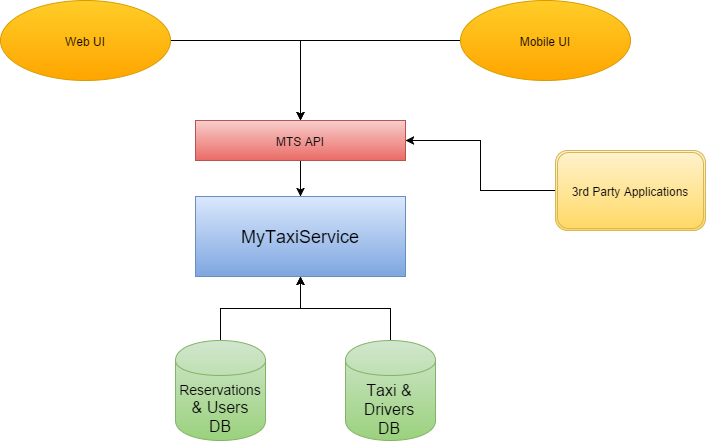
\includegraphics[width=0.84\columnwidth]{Blocchi Diagram (1)/Blocchi Diagram (1)}
\caption{Overall view of \textit{MyTaxiService} system}
\end{center}
\end{figure}

\subsection{Product functions}
The application will provide a set of functionalities for taxi reservations and also for saving money by sharing your ride. It will indeed be designed to improve the management of taxi queues in the various zones of the city and to decrease avarage customers' waiting time.\\
In order to implement a fair management of taxi queues the application will be based on taxis' locations.
The city is divided in zones of approximately 2 km$^2$ each and a queue is associated to every single zone.
The taxi availability is constantly communicated to the system through the driver mobile application. It can be in three different states: \textbf{free}, \textbf{shared} or \textbf{locked}.The taxi is set as \textit{free} as soon as the taxi driver logs into the application and goes back to this state when a ride is terminated.
When a taxi becomes available it is inserted in the right queue, depending on its GPS location.
When a ride request arrives, it is associated to a zone, depending on the starting address of the request, and the request is forwarded to the first taxi in the assigned zone's queue. If no taxi is available in that zone, the research is expanded to the adjacent zones.
If a taxi driver declines a request, his taxi will be put at the bottom of the queue.


\subsection{User characteristics}
\begin{itemize}
\item \textbf{Visitor}: a visitor is whoever opens the application without having been authenticated.
\item \textbf{Passenger}: a passenger is an authenticated user who is capable of reserving a ride from a certain location to another. He's also able to share a ride with other passengers or to look for shared rides.
\item \textbf{Taxi driver}: a taxi driver is an authenticated user who has been granted permissions to confirm or not a reservation when his taxi is \textit{free}. In case of confirmation he should list as \textit{busy} and will not receive any incoming reservations aside shared ones. In that case the taxi will become \textit{shared}.
\end{itemize}

\subsection{Constraints}
\subsubsection{Regulatory policies}
\textit{MyTaxiService} will be released on Google Play Store, Apple App Store and Windows Store and so it must respect their market policies.
\subsubsection{Hardware limitation}
\textit{MyTaxiService} will support only mobile devices newer than 2012.\\
The mobile application will be suitable for devices with screen sizes starting from 4.2{'}
\subsubsection{Interfaces to other applications}
\textit{MyTaxiService} is strongly dependent on MySQL as the main DBMS. It also uses PayPal as the only PSP.
\subsubsection{Parallel operation}
\textit{MyTaxiService} must support parallel operations on the same DB coming from both taxi drivers' and passengers' applications.
\subsubsection{Reliability requirements}
\textit{MyTaxiService} does not have reliability requirements.
\subsubsection{Criticality of the application}
The application doesn't have a critical role inside the taxi system, since any of the actions done by \textit{MyTaxiService}, can by accomplished by phone.
\subsubsection{Safety and security considerations}
Since the payments are processed externally and the data is handled by an external DBMS, there are no specific security issues.

\subsection{Assumptions and dependencies}
\begin{itemize}
\item \textbf{Taxi drivers must have a tablet} in order to use the application and to manage incoming calls.
\item \textbf{A standard user is whoever needs a taxi service} and is using the new available technology. \textbf{He must have a smartphone or a device with an internet access} so he can use either the web or the mobile application.
\item Web and mobile applications have the same functionalities aside the registration that is only available on the web.
\item \textbf{Users have a GPS-enabled devices}.
\item \textbf{At least a taxi is always available for a passenger}. It's not mandatory that it's available in the passenger request's area.
\end{itemize}

\subsection{Goals}
\begin{itemize}
\item {[}G1{]} Allow visitor to become a registered user (passenger).
\item {[}G2{]} Allow taxi drivers and passengers to log in into the application.
\item {[}G3{]} Allow passengers to request a taxi.
\item {[}G4{]} Allow passengers to see the code and the ETA of the incoming taxi.
\item {[}G5{]} Allow taxi drivers to accept or refuse a call.
\item {[}G6{]} Allow passengers to reserve a taxi for a certain time and place (origin and destination).
\item {[}G7{]} Send a confirm notification to the passenger and make a taxi \textit{busy} at least 10 minutes before the reservation time.
\item {[}G8{]} Allow a passenger to choose a shared ride.
\end{itemize}

\subsection{Apportioning of requirements}
List of possible future functions:
\begin{itemize}
\item Friends list and possibility to share rides specifically with them.
\item Possibility to cancel or modify a reservation.
\end{itemize}

\section{Scenarios}

\subsection{Scenario 1: Usage of the app}
Timmy needs a taxi to go back to his hotel in Sesame Street. So he picks up his phone and opens the \textit{MyTaxiService} app.
He is asked to allow the application to use his position and after that, he's asked to pick a destination. He writes "Sesame Street" and then he is asked to wait a moment.
After few seconds, a pop-up appears on the screen containing the taxi code, the EWT for the taxi, the ETA to home and the expected fare.
He waits for the taxi to arrive and after he's back home, he's notified of the fare which is directly drawn from his credit card.

\subsection{Scenario 2: Taxi reservation}
Bob is abroad on holiday and is going to take a plane to go back to his city, but he realizes that no one can take him back home from the airport, so he decides to book a taxi ride. His smartphone is dead so he turns on his laptop, connects to the airport's Wi-Fi and opens the \textit{mytaxiservice.com} website. He signs in with his credentials and opens the \textit{"New Ride"} view. He selects the starting place(the airport), the destination ("21st avenue"), and chooses the departing time. During his flight he charges his mobile phone so when he lands he turns on his phone and receives all the information about his reservation. At the booked time the taxi arrives and brings him home. The taxi driver communicates him the ride fare and he pays in cash.

\subsection{Scenario 3: Shared ride, passenger's side}
Penny bought a ticket to go to the theater for a new musical. She decides to go with a taxi but she wants to save money because she has already spent a lot for the show ticket. So she opens the \textit{myTaxiService} application and chooses a shared ride for the theater.
In the meanwhile Leonard realizes he has to go to a restaurant near the theater for a dinner with his colleagues but his car is broken. So he picks up his mobile phone and opens the \textit{myTaxiService} app. He decides to choose a shared ride to save some money so he selected the option and confirms.
Both Penny and Leonard receive the information of the same taxi for their ride. The taxi first stops at Leonard's home and the taxi driver tells him that his ride is shared and he will stop to take another passenger. The taxi stops after a few minutes at Penny's home and then it takes them to their destination. Once arrived the taxi driver tells them their respectively fares and they pay.

\subsection{Scenario 4: Shared ride, driver's side}
Walter White, a taxi driver for the \textit{myTaxiService} company, is driving along "Main Street" when he receives a notification from the taxi application for a shared ride. He accepts the request and goes at the given address in order to pick up the passenger. After driving for a few minutes he receives another request so he stops to pick up three other passengers and his car is now full. He drives to the first destination, selects the "Terminate Ride" button and tell the passenger the fare that will be charged on his PayPal account. Then he drives to the last stop and leaves the other passengers, he takes the payment in cash and terminate the current ride on the app.

\subsection{Scenario 5: Taxi driver notifications}
Jack Tahyer is a taxi driver and he has to put \textit{myTaxiService} onto his mobile. He is bottled up in traffic due to a car accident. He receives a notification for a new passenger but it would take too much time to reach the customer so he decides to decline the request. After some time he finally has open road and he receives another request for a shared ride. He accepts the request and follows the GPS directions.

\section{Specific requirements}
In this section detailed descriptions of the functional and quality requirements will be presented together with the explicit features requested.
\subsection{External interface requirements}
In the paragraphs below an analysis of inputs and outputs of the system will be presented both from the user and software perspectives.
\subsubsection{User interfaces}
The first view a user should see is the "Sign In" page both from mobile and web apps.
Then, if it's their first time within the application, the user should move to the sign up page, in order to begin the registration process.
\newpage

% ---------------------- Mobile Login Image Block ---------------------- %
\begin{figure}
    \centering
    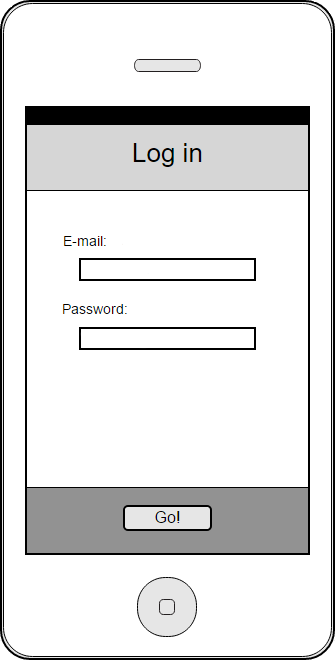
\includegraphics[width=0.35\columnwidth]{Login1/Login1}
    \caption{Login page for mobile application}
    \label{fig:mobile-login}
\end{figure}
% ---------------------------------------------------------------------- %

% -------------------- Web Registration Image Block -------------------- %
\begin{figure}[h!]
    \centering
    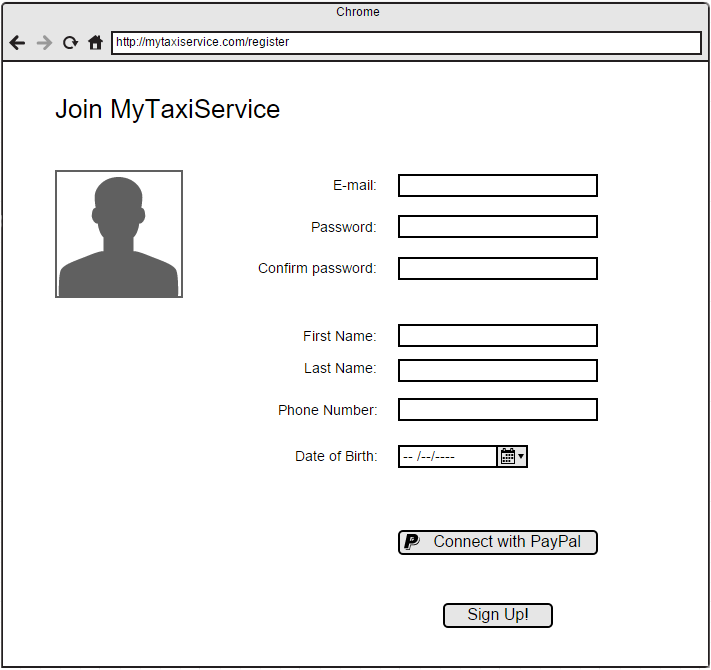
\includegraphics[width=0.5\columnwidth]{Register/Register}
    \caption{Web registration page}
    \label{fig:web-register}
\end{figure}
% ---------------------------------------------------------------------- %

\newpage

If however they already have an account, after the sign in process:
\begin{itemize}
    
    \item If the user is a \textbf{passenger}, they will see the \textit{Home} page which contains a brief log of his rides and an option to begin a \textit{new ride}.
% ------------------ Mobile History Rides Image Block ------------------ %
\begin{figure}[h!]
    \centering
    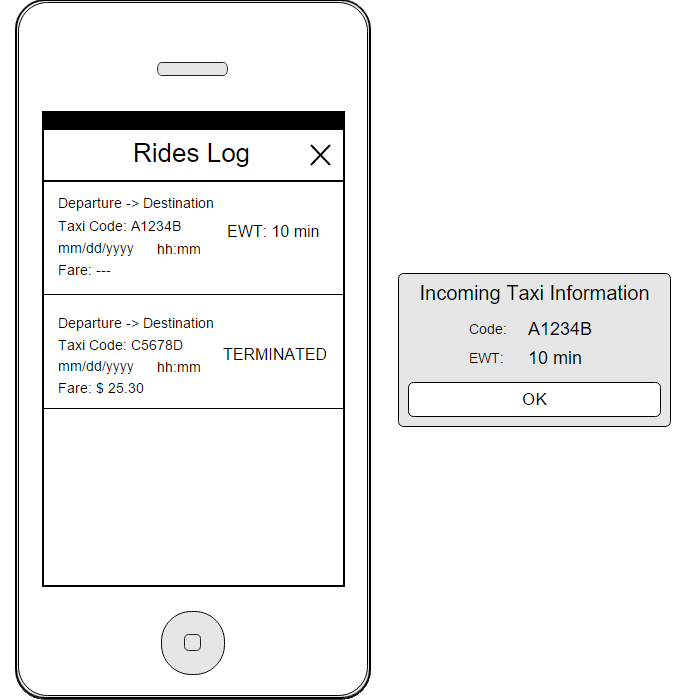
\includegraphics[width=0.56\columnwidth]{informations1/informations}
    \caption{Rides informations}
    \label{fig:mobile-ride_info}
\end{figure}
% ---------------------------------------------------------------------- %
% --------------------- Mobile New Ride Image Block -------------------- %
    \begin{figure}[h!]
        \centering
        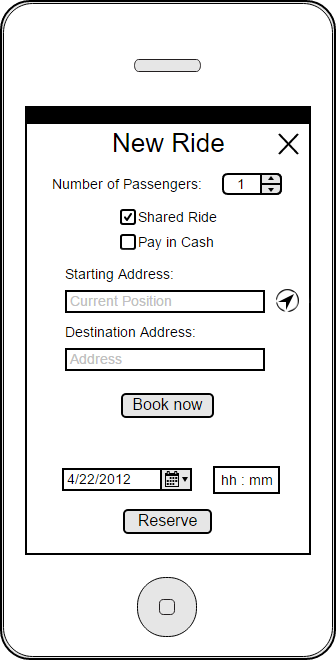
\includegraphics[width=0.308\columnwidth]{New Ride/New Ride}
        \caption{New Ride page}
        \label{fig:mobile-new_ride}
    \end{figure}
% ---------------------------------------------------------------------- %

\newpage
    
    \item If instead the user is a \textbf{taxi driver} then they will directly see the \textit{Driver} page which shows recent notifications and a map with the route to the next destination \textit{(Figure 6)}. If a shared ride is accepted the interface changes \textit{(Figure 7)} showing all the passengers that have booked the shared ride and the possibility to terminate the ride for a single user. When a ride is terminated, for both normal and shared rides, a notification pops up \textit{(Figure 8)} showing the fare that should be payed and the payment method chosen by the passenger.
% ----------------- Tablet Driver Interface Image Block ---------------- %
    \begin{figure}[h!]
        \centering
        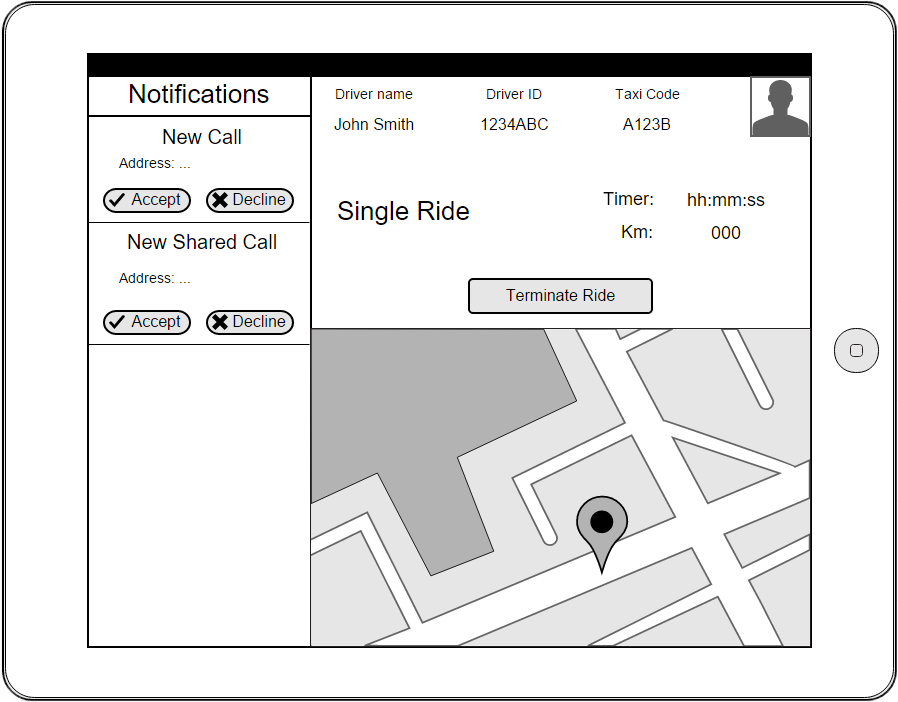
\includegraphics[width=0.7\columnwidth]{driver/driver}
        \caption{Taxi Driver interface}
        \label{fig:tablet-driver}
    \end{figure}
    
    \begin{figure}[h!]
        \centering
        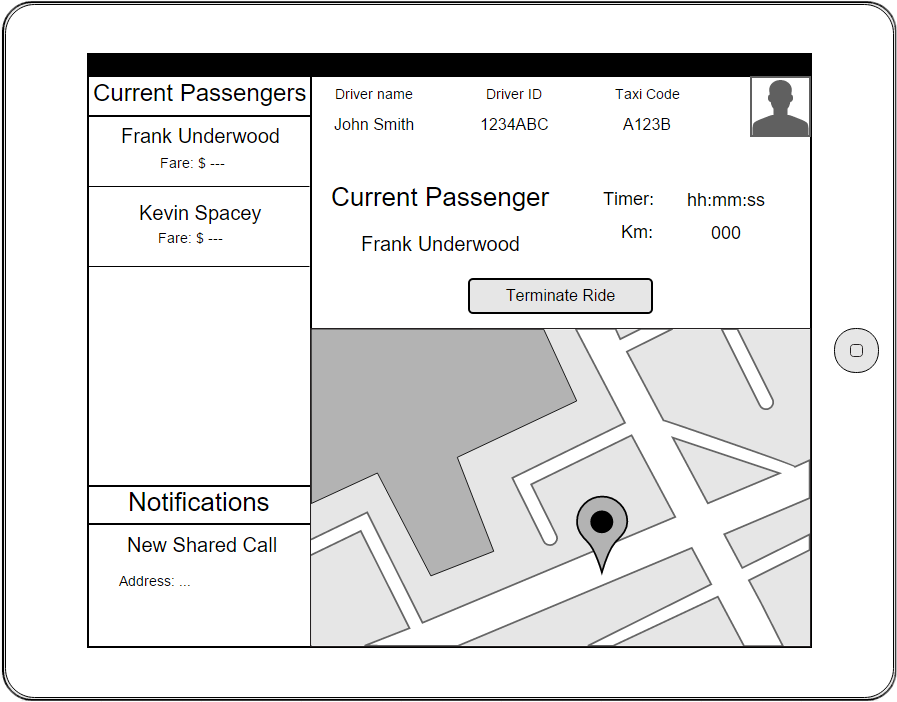
\includegraphics[width=0.7\columnwidth]{driver/driver-shared}
        \caption{Taxi Driver interface for shared ride}
        \label{fig:tablet-driver-shared}
    \end{figure}
    
    \begin{figure}[h!]
        \centering
        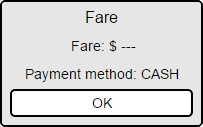
\includegraphics[width=0.3\columnwidth]{driver/driver-fare}
        \caption{Notification for terminated ride}
        \label{fig:driver-notification}
    \end{figure}
% ---------------------------------------------------------------------- %
\newpage

\end{itemize}

\subsubsection{Hardware interfaces}
Since the application is compliant to modern standards, there is no specific limitation on the hardware itself. The only limitation to use the app is that it must be used from a GPS enabled device.

\subsubsection{Communication interfaces}
Since both the front-end and the back-end are being developed from scratch, there are no specific restrictions on the communication between system components except from the underlying data layer which will be discussed later.

\subsubsection{Software interfaces}
The system has to interact with a preexisting database containing taxis and drivers.
The application also provides public API for further and additional integration.

\newpage
\subsection{Functional requirements}

\subsubsection{User 1 - Visitor}
\begin{enumerate}
\item \textit{\textbf{Registering}} - \textbf{[G1]}\\*
A visitor can register into the application by compiling the registration form.\\*\\*
Requirements:
\begin{enumerate}
\item Visitor must enter a valid email.
\item Visitor must enter a valid phone number.
\item Visitor must be adult in order to register.
\end{enumerate}
\end{enumerate}

\subsubsection{User 2 - Passenger}

\begin{enumerate}
\item \textit{\textbf{Connect to PayPal}}\\
A passenger can connect his account to PayPal. The application will ask permissions to use passenger's PayPal account.
\item \textit{\textbf{Pay with PayPal}}\\
A passenger can pay a ride with PayPal.\\
Requirements:
\begin{enumerate}
\item Passenger must have connected his account with PayPal.
\end{enumerate}

\item \textit{\textbf{Login}} - \textbf{[G2]}\\
A passenger has to login in order to access to all the other passenger functions.

\item \textit{\textbf{Request a new taxi ride}} - \textbf{[G3, G6, G8]}\\*
A passenger can book a taxi. He will have to fill the following input information: starting point (automatically filled if GPS is enabled) and destination.\\
Requirements:
\begin{enumerate}
\item A passenger must have not requested another taxi at the same time.
\end{enumerate}
Domain properties:
\begin{enumerate}
\item Starting place must be in the city in which the service is being deployed.
\item Destination place must be in the country.
\end{enumerate}
There are some particular cases:
\begin{itemize}
\item Shared taxi ride: request for a new shared ride.
\item Reservation: passenger will have to add a booking date and the starting point if auto-fill is disabled.\\
Additional domain properties:
\begin{enumerate}
\item The ride time must be in the future within a month and at least 2 hours from current time.
\end{enumerate}
\end{itemize}

\iffalse
\item \textit{\textbf{Request a new standard taxi ride}} - \textbf{[Goal 3]}\\*
A passenger can ask for an immediate ride. He will have to fill the following input information: starting point (automatically filled if GPS is enabled) and destination.\\
Requirements:
\begin{enumerate}
\item A passenger must have not requested another taxi at the same time.
\end{enumerate}
Domain properties:
\begin{enumerate}
\item Starting place must be in the interested city.
\item Destination place must be in the country.
\end{enumerate}

\item \textit{\textbf{Request a new shared taxi ride}} - \textbf{[G8]}\\*
A passenger can ask for a shared taxi ride in order to save money or have company.\\
Requirements:
\begin{enumerate}
\item A passenger must have not request another taxi at the same time.
\end{enumerate}
Domain properties:
\begin{enumerate}
\item Starting place must be in the interested city.
\item Destination place must be in the country.
\end{enumerate}

\item \textit{\textbf{Book a new taxi ride}} - \textbf{[G6]}\\*
A passenger can ask for a future ride. He will also have to add a date. The starting point's auto-fill is disabled.\\
Requirements:
\begin{enumerate}
\item A passenger must have not request another taxi at the same time.
\end{enumerate}
Domain properties:
\begin{enumerate}
\item Starting place must be in the interested city.
\item Destination place must be in the country.
\item Booking time must be in the future within a month and at least 2 hour from actual time.
\end{enumerate}
\fi

\item \textit{\textbf{Look rides log}} - \textbf{[G4]}\\
A passenger can look at all his rides. They have a taxi ID (besides future rides), a fare (besides current and future rides), a starting and an ending place.\\
Requirements:
\begin{enumerate}
\item Passenger must have booked at least one ride.
\end{enumerate}
\end{enumerate}

\subsubsection{User 3 - Taxi driver}
\begin{enumerate}

\item \textit{\textbf{Manage a ride notification}} - \textbf{[G5]}\\*
A taxi driver can accept a ride notification. The application will show taxi information to the passenger and it will prevent the driver to receive any new standard ride notification  (i.e. \textit{busy}).\\
Requirements:
\begin{enumerate}
\item The taxi related to the driver is not \textit{busy} or \textit{shared}.
\end{enumerate}
Domain property:
\begin{enumerate}
\item Maximum number of passengers is 4.
\end{enumerate}
There are some particular cases:
\begin{itemize}
\item Accept a shared ride notification: the taxi is \textit{shared} instead of \textit{busy}.\\
Additional requirements:
\begin{enumerate}
\item No passenger must be in the car. Besides the first shared ride notification, the others are automatically accepted until the end of the ride.
\end{enumerate}
\item Decline a ride notification: the taxi driver can decline a ride request.\\
Additional requirements:
\begin{enumerate}
\item Taxi must not be \textit{shared}.
\end{enumerate}
\end{itemize}

\iffalse
\item \textit{\textbf{Accept a regular ride notification}} - \textbf{[G5]}\\*
A taxi driver can accept a regular ride notification. The application will send the taxi data to the passenger and will prevent the driver to receive any other notification (\textit{lock}).\\
Requirements:
\begin{enumerate}
\item The taxi related to the taxi driver is not locked or shared.
\end{enumerate}
Domain property:
\begin{enumerate}
\item Maximum number of passenger is 4.
\end{enumerate}

\item \textit{\textbf{Accept a shared ride notification}} - \textbf{[G5]}\\*
A taxi driver can accept a shared ride notification. The application will send the taxi data to the passenger and will enable just the receiving of other shared ride (\textit{share lock}).\\
Requirements:
\begin{enumerate}
\item No passenger must be in the car. Besides the first shared ride notification, the others are automatically accepted until the end of the ride.
\item The taxi related to the taxi driver is not locked.
\end{enumerate}
Domain property:
\begin{enumerate}
\item Maximum number of passenger is 4.
\end{enumerate}

\item \textit{\textbf{Decline a ride}} - \textbf{[G5]}\\*
A taxi driver can decline a ride request.\\
Requirements:
\begin{enumerate}
\item Taxi must not be shared.
\end{enumerate}
\fi

\item \textit{\textbf{Start a ride}}\\
A taxi driver can start a ride for a passenger.\\
Requirements:
\begin{enumerate}
\item There must be a pending request from the passenger.
\end{enumerate}

\item \textit{\textbf{Finish a ride}}\\*
A taxi driver can finish a ride. The application will show the final fare and distance and will \textit{free} the taxi.\\
Requirements:
\begin{enumerate}
\item The taxi related to the taxi driver is \textit{busy} or \textit{shared}.
\item The ride must have been started.
\end{enumerate}

\end{enumerate}



\subsection{Use Cases}
In this sections a UML Use Case Diagram will be presented, giving a general idea of the application features and then some features will be analyzed more in detail by UML Sequence Diagrams.  

\subsubsection{Visitor registration}
\begin{tabular}{| l | p{8cm} |}
\hline
\textbf{Actor}      &       Visitor \\
\hline
\textbf{Goal}       &       [G1]\\
\hline
\textbf{Entry Condition} &  NULL\\
\hline
\textbf{Event Flow}     &   1.	Visitor opens the registration page.\\&
                                            2.	Visitor fills all the fields.\\&
                                            3.	Visitor confirms the registration clicking on “Sign Up!”.\\&
                                            4.  The data is checked.\\&
                                            5.	The data is registered.\\
\hline
\textbf{Output Condition} & Visitor successfully registers and becomes a passenger. From now on he can log into the application.\\
\hline
\textbf{Exceptions} &       •   One or more fields are empty.\\& 
                            •	Email is already associated to another account.\\&
                            •	Password doesn't respect the constraints.\\& 
                            All the exceptions are handled by notifying to the visitor the occurred problem and resetting the form.\\
\hline
\end{tabular} 

\subsubsection{Login}
\begin{tabular}{| l | p{8cm} |}
\hline
\textbf{Actor}      &       User, Visitor \\
\hline
\textbf{Goal}       &       [G2]\\
\hline
\textbf{Entry Condition} &  The user is already registered.\\
\hline
\textbf{Event Flow}     &  1.	The visitor opens the \textit{login} page.\\&
                                            2.	The visitor fills the email and password fields.\\&
                                            3.  The visitor confirms clicking on “Go!”.\\&
                                            4.	The user is redirected at the personal page.
\\
\hline
\textbf{Output Condition} & The registered user is now logged in and has access to his personal features.\\
\hline
\textbf{Exceptions} &       •	One or both email and password are wrong or empty.\\&
                            The exception is handled by notifying to the user the occurred problem and resetting the form.
\\
\hline
\end{tabular} 


\subsubsection{Standard request}
\begin{tabular}{| l | p{8cm} |}
\hline
\textbf{Actor}      &       Passenger \\
\hline
\textbf{Goal}       &       [G3]\\
\hline
\textbf{Entry Condition} &  The passenger is logged in.\\
\hline
\textbf{Event Flow}     &  1.	Passenger opens the “New Ride” page.\\&
                                            2.	Passenger fills the addresses fields, selects the number of passengers and unchecks the \textit{Shared Ride} option.\\&
                                            3.	Passenger confirms clicking on “Book Now”.\\
\hline
\textbf{Output Condition} & The request is sent and the passenger waits for the taxi information.\\
\hline
\textbf{Exceptions} &       •	One or more fields are empty or invalid.\\&

The passenger is notified of the occurred problem and the form is reset.\\&
• No taxi driver is found in the area.\\&
The system looks for a taxi in the nearest areas around the interested one.\\
\hline
\end{tabular} 


\subsubsection{Rides Log}
\begin{tabular}{| l | p{8cm} |}
\hline
\textbf{Actor}      &       Passenger \\
\hline
\textbf{Goal}       &       [G4]\\
\hline
\textbf{Entry Condition} &  The passenger is logged in.\\&
                            The passenger has booked or reserved a ride.\\
\hline
\textbf{Event Flow}     &  1.	The passenger opens the \textit{Rides Log} page.\\
\hline
\textbf{Output Condition} & The passenger has access to the incoming taxi information and to all of his previous rides.\\
\hline
\textbf{Exceptions} &       NULL\\
\hline
\end{tabular} 

\subsubsection{Taxi reservation}
\begin{tabular}{| l | p{8cm} |}
\hline
\textbf{Actor}      &       Passenger \\
\hline
\textbf{Goal}       &       [G6]\\
\hline
\textbf{Entry Condition} &  The passenger is logged in.\\
\hline
\textbf{Event Flow}     & 1.	The passenger opens the “New Ride” page.\\&
                                            2.	The passenger fills the addresses fields, selects the number of passengers, unchecks the \textit{Shared Ride} option and selects date and time for the reservation.\\&
                                            3.	The passenger confirms clicking on “Reserve”.\\
\hline
\textbf{Output Condition} & The request is sent and it will be processed 10 minutes before the reservation time.\\
\hline
\textbf{Exceptions} &      •	One or more fields are empty.\\&
      •	The ride time is less then two hours from the current time.\\&
The exception is handled by notifying to the user the occurred error and resetting the form.\\
\hline
\end{tabular}

\subsubsection{Taxi reservation (already booked)}
\begin{tabular}{| l | p{8cm} |}
\hline
\textbf{Actor}      &       Passenger, Taxi driver \\
\hline
\textbf{Goal}       &       [G5], [G7]\\
\hline
\textbf{Entry Condition} &  The passenger is logged in.\\&
The taxi driver is logged in.\\&
                            There is a pending taxi request from the passenger for the next 10 minutes.\\
\hline
\textbf{Event Flow}     & 1.	The system searches a taxi in the requested location area.\\&
                                            2.	A notification is sent to the taxi driver found.\\&
                                            3.	The taxi driver accepts the call.\\&
                                            4.	The EWT is calculated.\\&
                                            5.	The taxi ID code and the EWT are sent to the passenger.
\\
\hline
\textbf{Output Condition} &     The request is sent and the passenger receives the taxi information.\\
\hline
\textbf{Exceptions} &      • No taxi driver is found in the area.\\&
The system looks for a taxi in the nearest areas around the interested one.\\&
• The taxi driver declines the call.\\&

The exception is handled searching for another taxi in the area and restarting from the event flow's point 2.\\
\hline
\end{tabular} 

\subsubsection{Shared Ride request}
\begin{tabular}{| l | p{8cm} |}
\hline
\textbf{Actor}      &       Passenger \\
\hline
\textbf{Goal}       &       [G8]\\
\hline
\textbf{Entry Condition} &  The passenger is logged in.\\
\hline
\textbf{Event Flow}     & 1.	The passenger opens the “New Ride” page.\\&
                                            2.	The passenger fills the addresses fields, selects the number of passengers, checks the \textit{Shared Ride} option and selects date and time for the reservation.\\&
                                            3.	The passenger confirms clicking on “Reserve”.\\
\hline
\textbf{Output Condition} & The request is sent and the passenger waits for the taxi information.\\
\hline
\textbf{Exceptions} &     •	One or more fields are empty or invalid.\\&

The passenger is notified of the occurred problem and the form is reset.\\&
• No taxi driver is found in the area.\\&
The system looks for a taxi in the nearest areas around the interested one.\\
\hline
\end{tabular}

\subsubsection{Ride management and completion}
\begin{tabular}{| l | p{8cm} |}
\hline
\textbf{Actor}      &       Taxi driver \\
\hline
\textbf{Goal}       &       NULL\\
\hline
\textbf{Entry Condition} &  The passenger has requested a ride.\\& The pointed out taxi in the notification arrives at the established location.\\
\hline
\textbf{Event Flow}     &           1.	The driver starts the ride by clicking on "Start Ride" when the passenger gets in the taxi .\\&
                                    2.	The driver takes the passenger to the destination.\\&
                                    3.	The driver clicks on "Terminate Ride".\\&
                                    4.  A notification appears showing the total fare that has to be payed and the payment method chosen by the passenger during the reservation phase.\\
\hline
\textbf{Output Condition} & The taxi is now available in his current area and the taxi driver can receive notifications for new rides.\\
\hline
\textbf{Exceptions} &    NULL\\
\hline
\end{tabular}

\subsubsection{Shared ride management}
\begin{tabular}{| l | p{8cm} |}
\hline
\textbf{Actor}      &       Taxi driver \\
\hline
\textbf{Goal}       &       NULL\\
\hline
\textbf{Entry Condition} &  A passenger booked a shared ride and he's already on board.\\
\hline
\textbf{Event Flow}     &           1. The driver receives a new shared ride call.\\&
                                    2. The new passenger is added to the \textit{Current Passengers} of the taxi.\\&
                                    3. The driver gets to the new address to take the new passenger.\\&
                                    4. The second ride is started when the new passenger gets in the taxi.\\&
                                    5. The \textit{Current Passenger} is automatically set to the first passenger that will leave the taxi\\&
                                    6. The driver takes the first passenger to the destination and terminates his ride.\\&
                                    7. A notification appears showing the total fare that has to be payed and the payment method chosen by the passenger during the reservation phase.\\
\hline
\textbf{Output Condition} & The taxi is still shared with other passenger on board.\\
\hline
\textbf{Exceptions} &    NULL\\
\hline
\end{tabular}

\newpage


\begin{landscape}

\vfill
    \begin{figure}[h!]
        \centering
        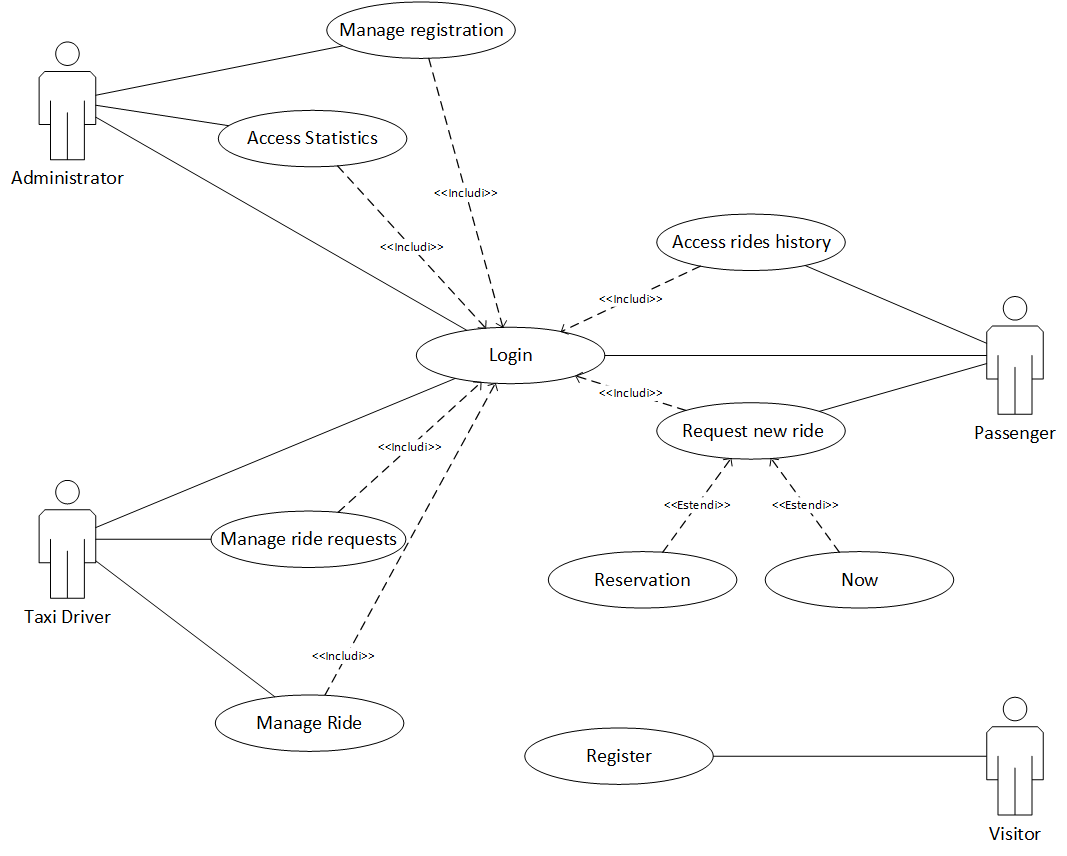
\includegraphics[width=0.75\columnwidth]{UseCase/UCDiagram}
        \caption{Use Case Diagram of the whole application usage}
        \label{fig:usecase}
    \end{figure}
    \vfill
 \end{landscape}
 
     \begin{figure}[h!]
        \centering
        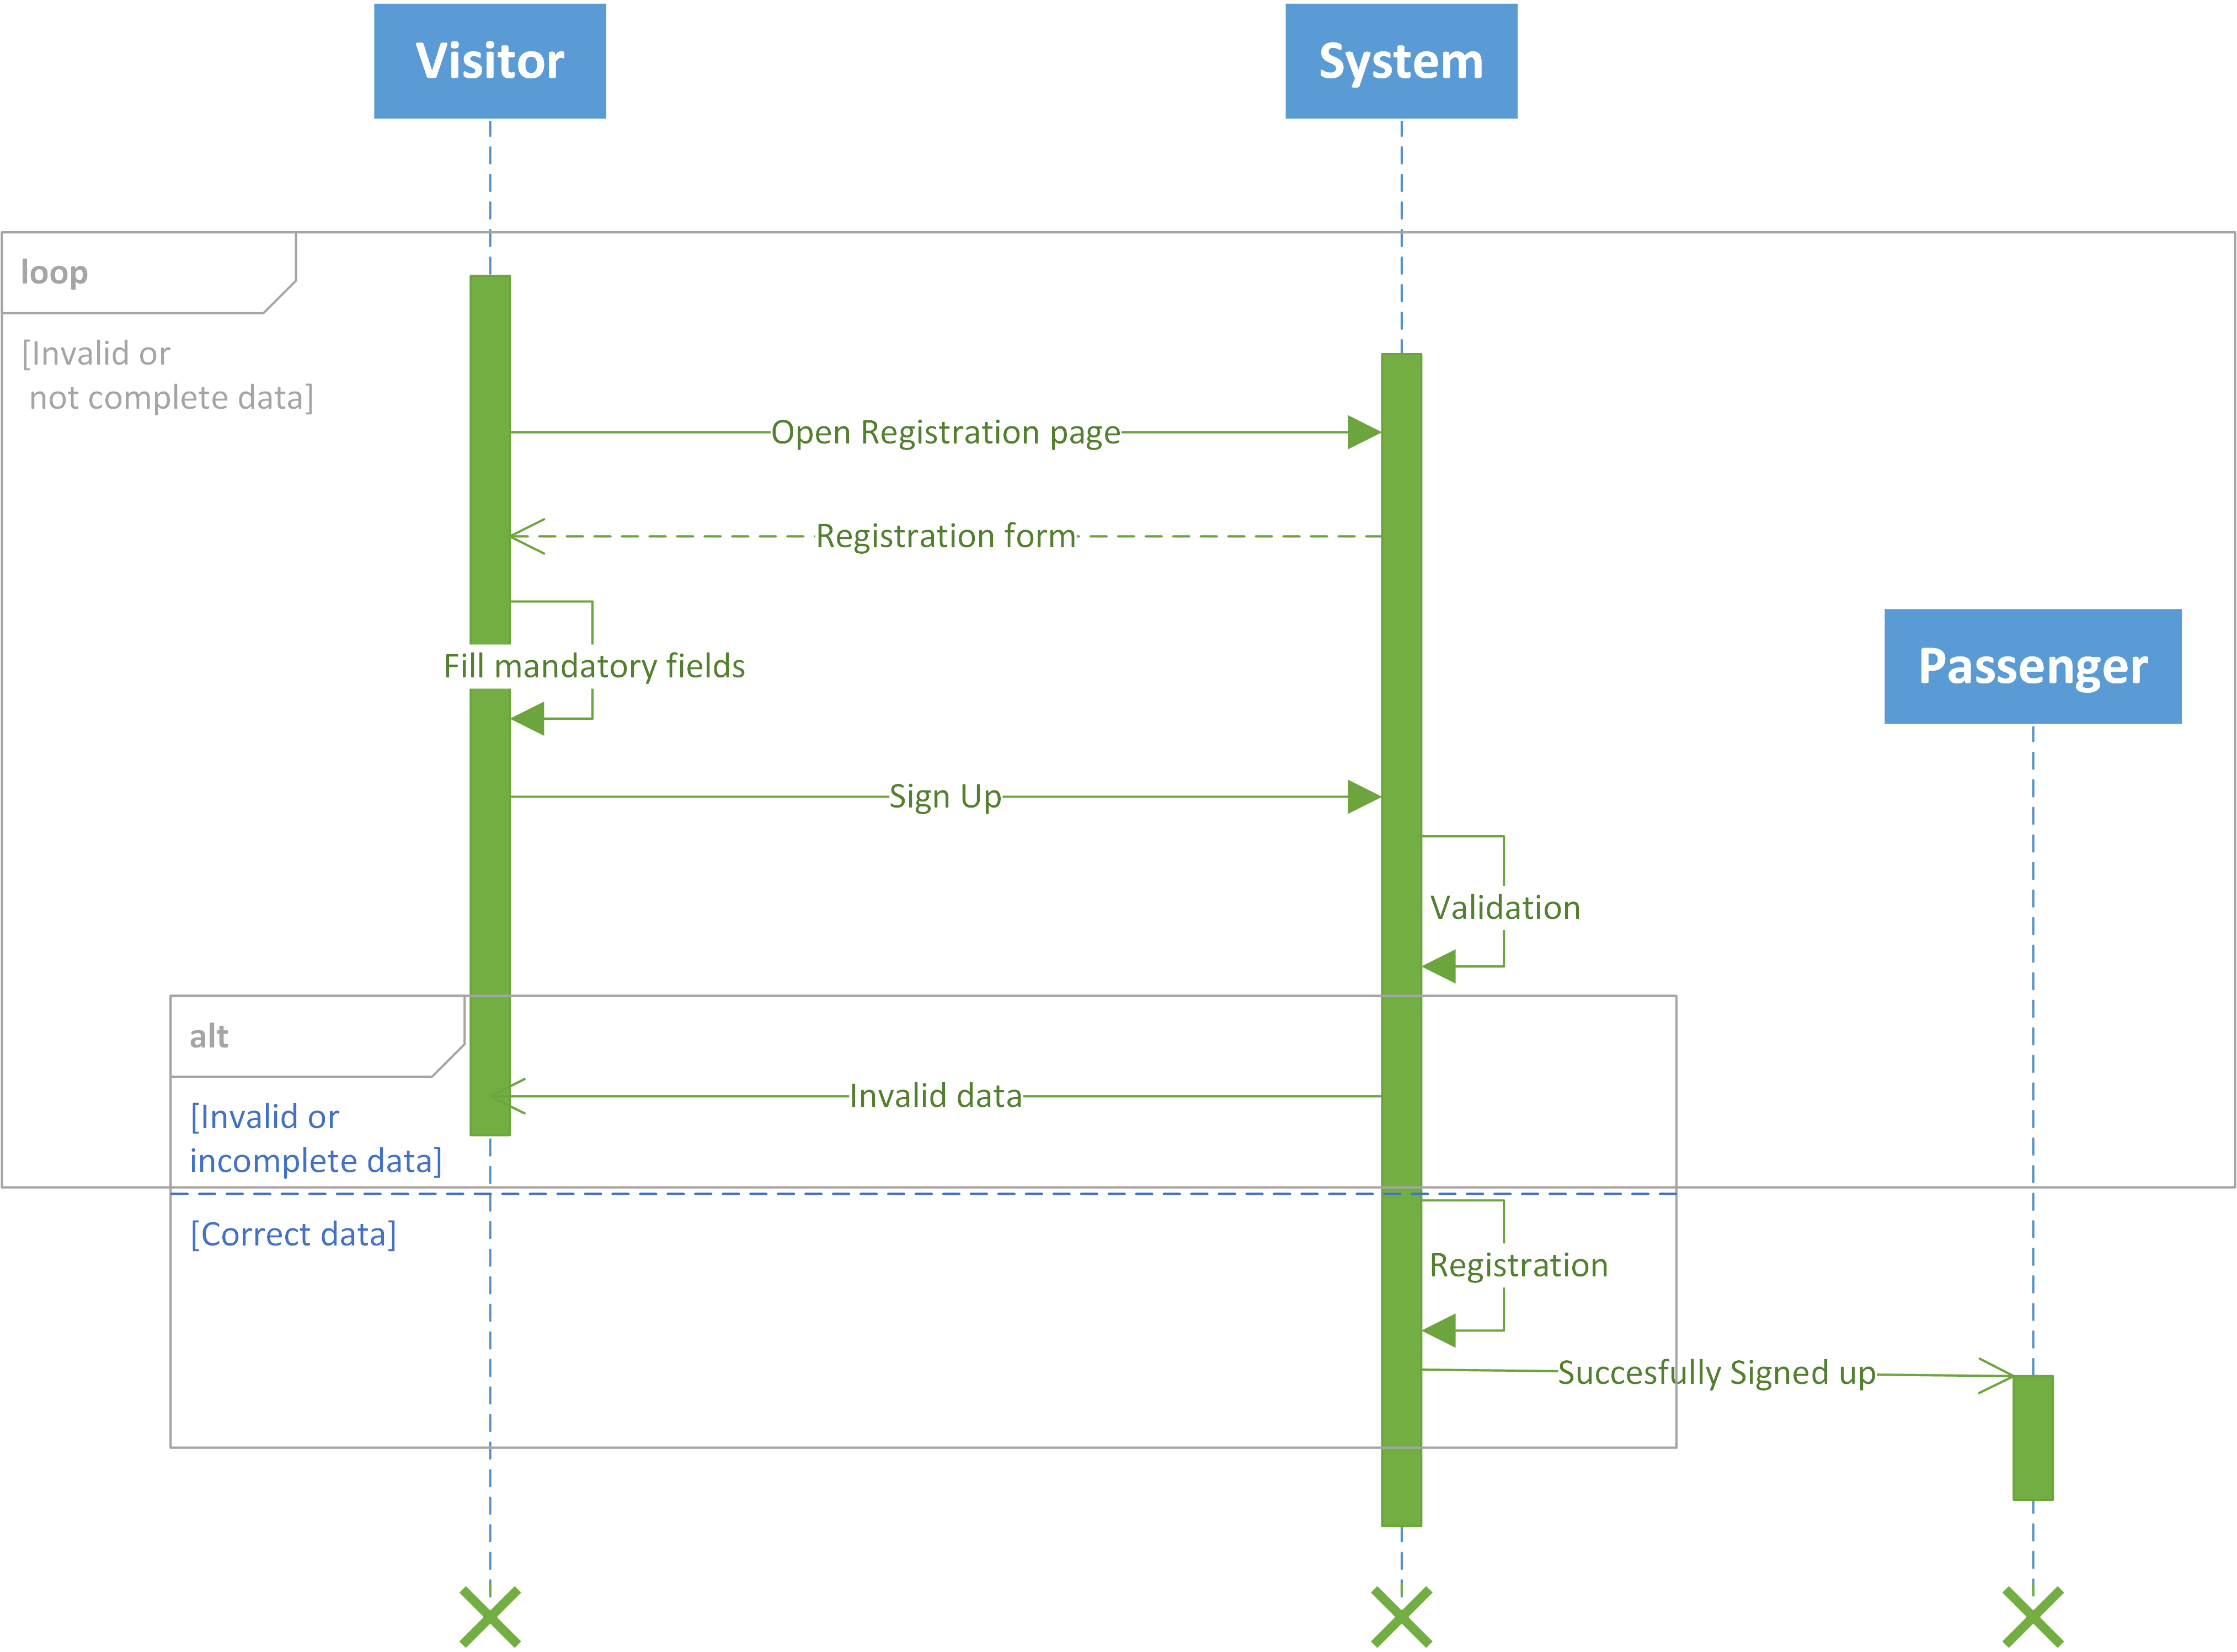
\includegraphics[width=1\columnwidth]{sequenceDiagram/registration}
        \caption{Registration process - Use case 4.3.1}
        \label{fig:seq-reg}
    \end{figure}
    
    \begin{figure}[h!]
        \centering
        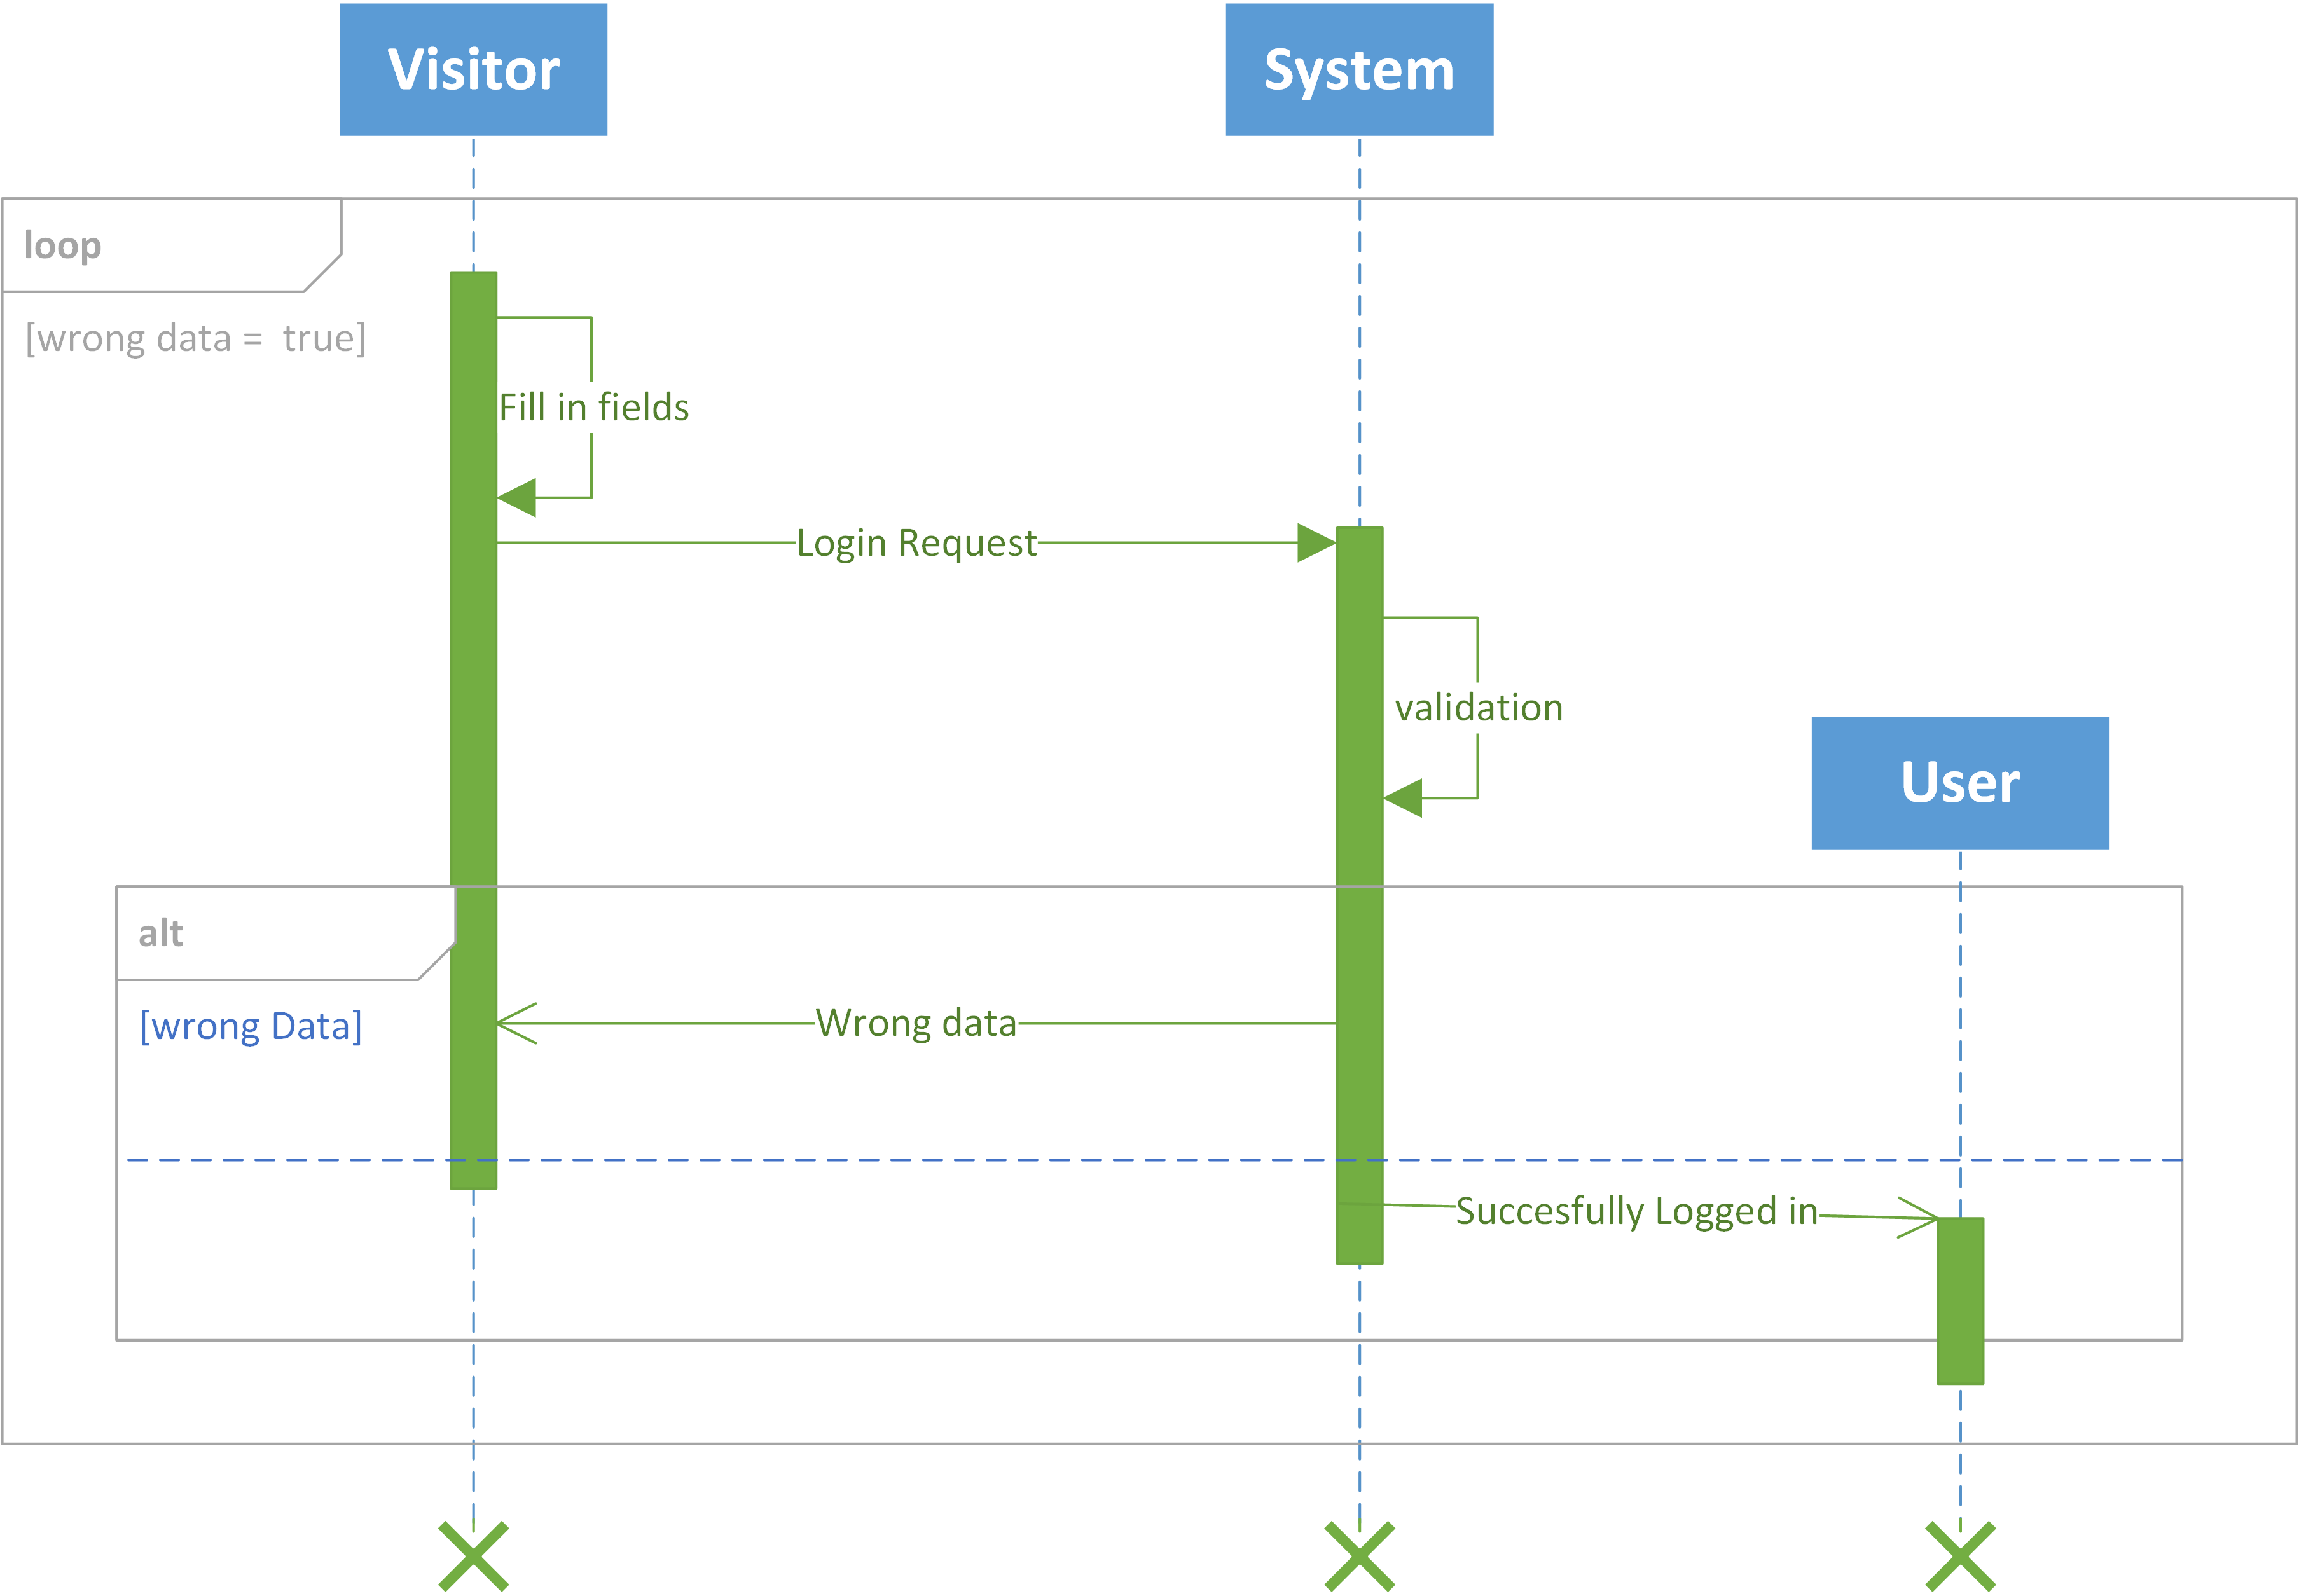
\includegraphics[width=1\columnwidth]{sequenceDiagram/Login}
        \caption{Login process - Use case 4.3.2}
        \label{fig:seq-login}
    \end{figure}


        \begin{figure}[h!]
        \centering
        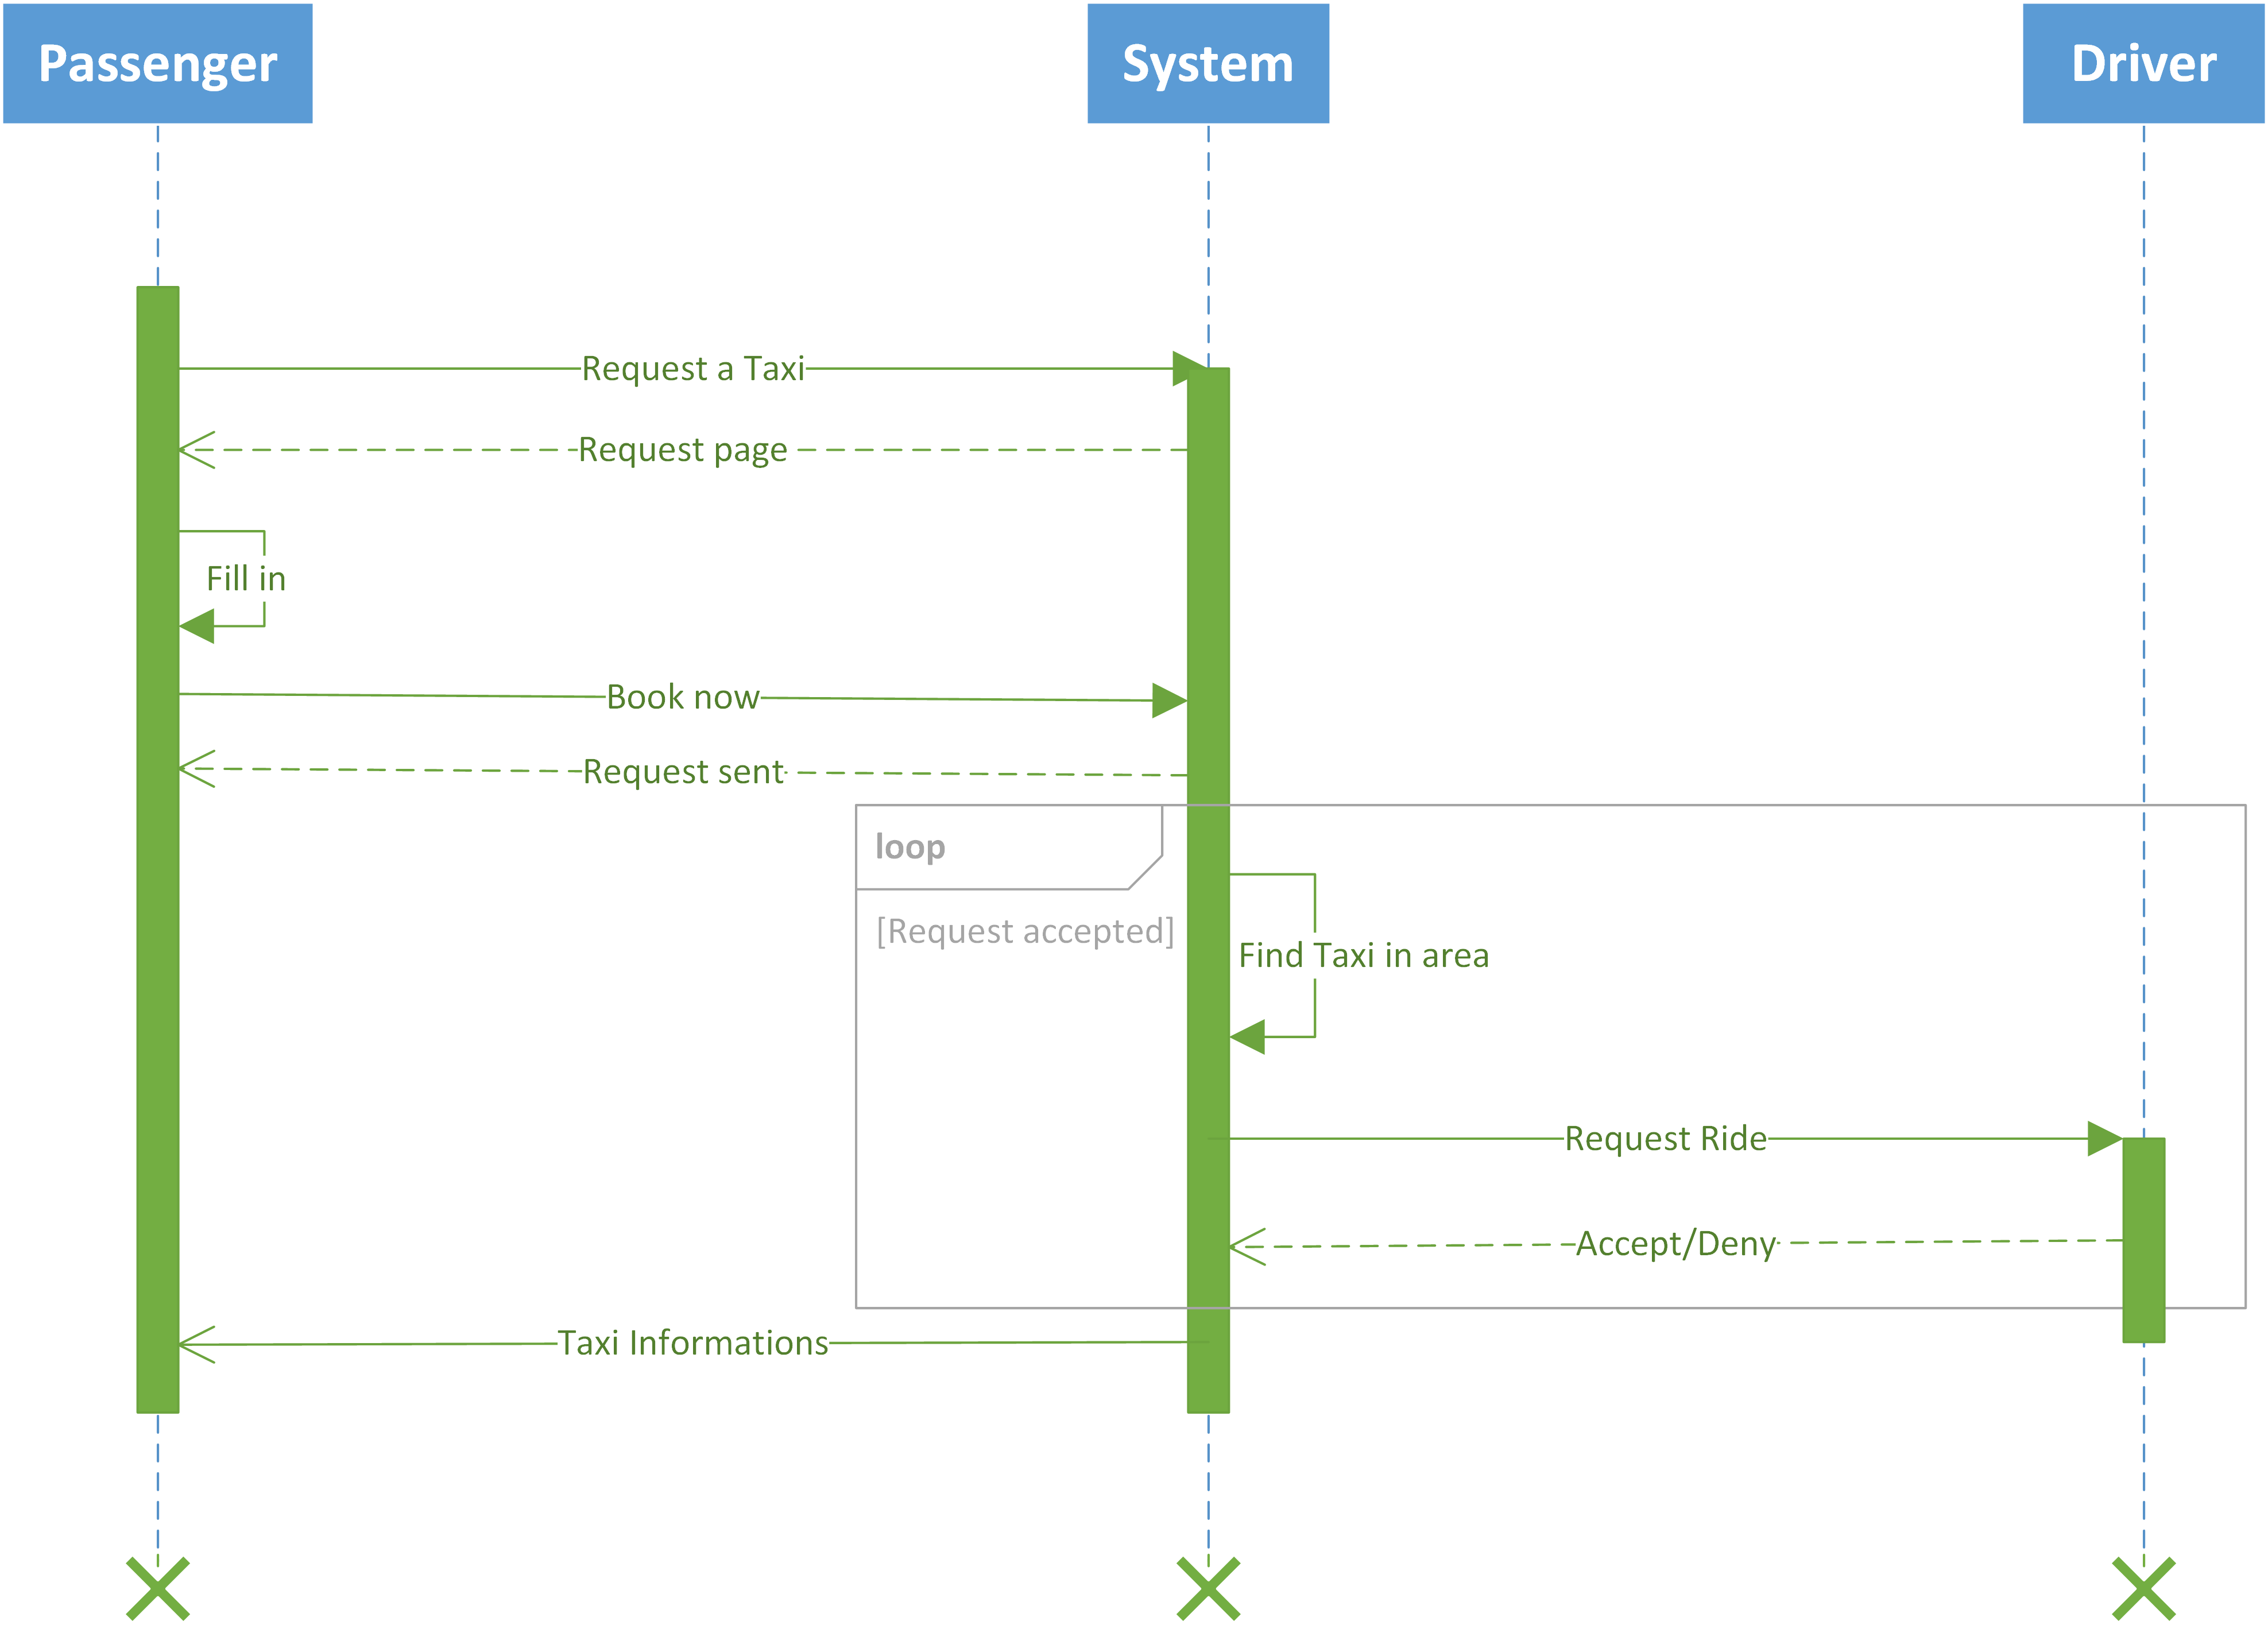
\includegraphics[width=1\columnwidth]{sequenceDiagram/sequence-request}
        \caption{Taxi request process - Use case 4.3.3/5 and 4.3.6}
        \label{fig:seq-req}
    \end{figure}

\newpage 

        \begin{figure}[h!]
        \centering
        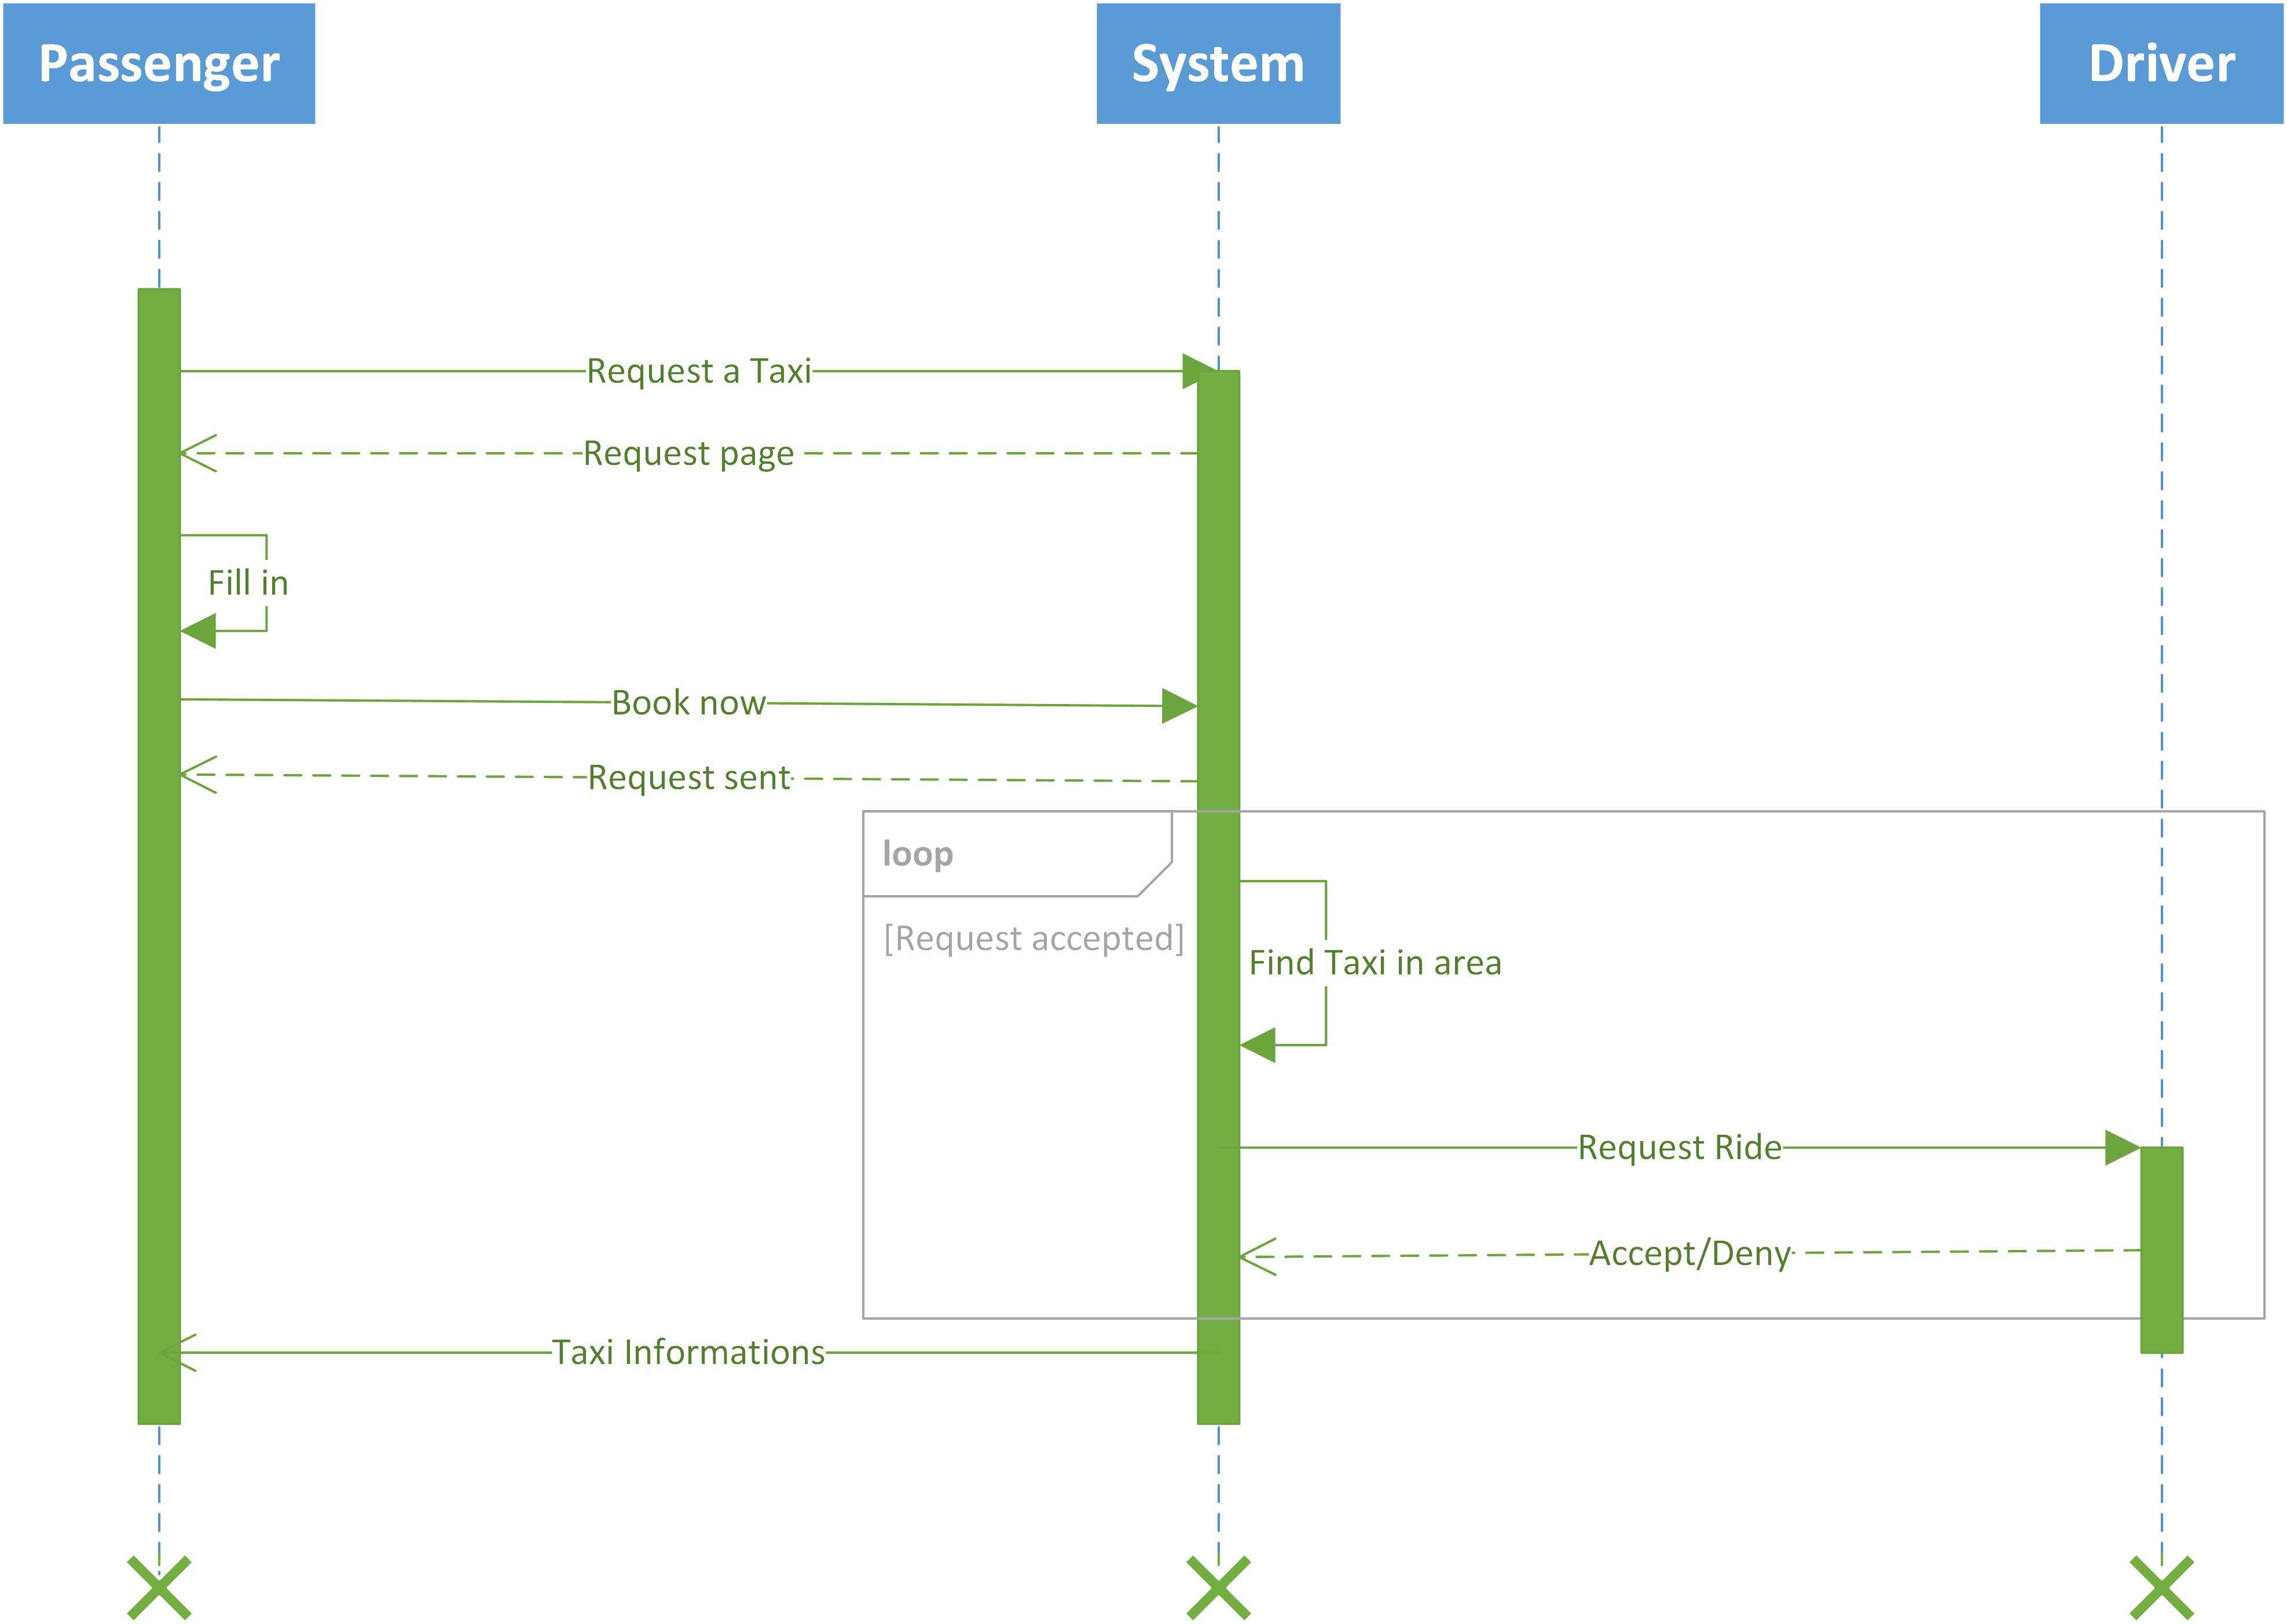
\includegraphics[width=1\columnwidth]{sequenceDiagram/shared-request}
        \caption{Shared taxi request process - Use case 4.3.7}
        \label{fig:seq-shreq}
    \end{figure}
    

        \begin{figure}[h!]
        \centering
        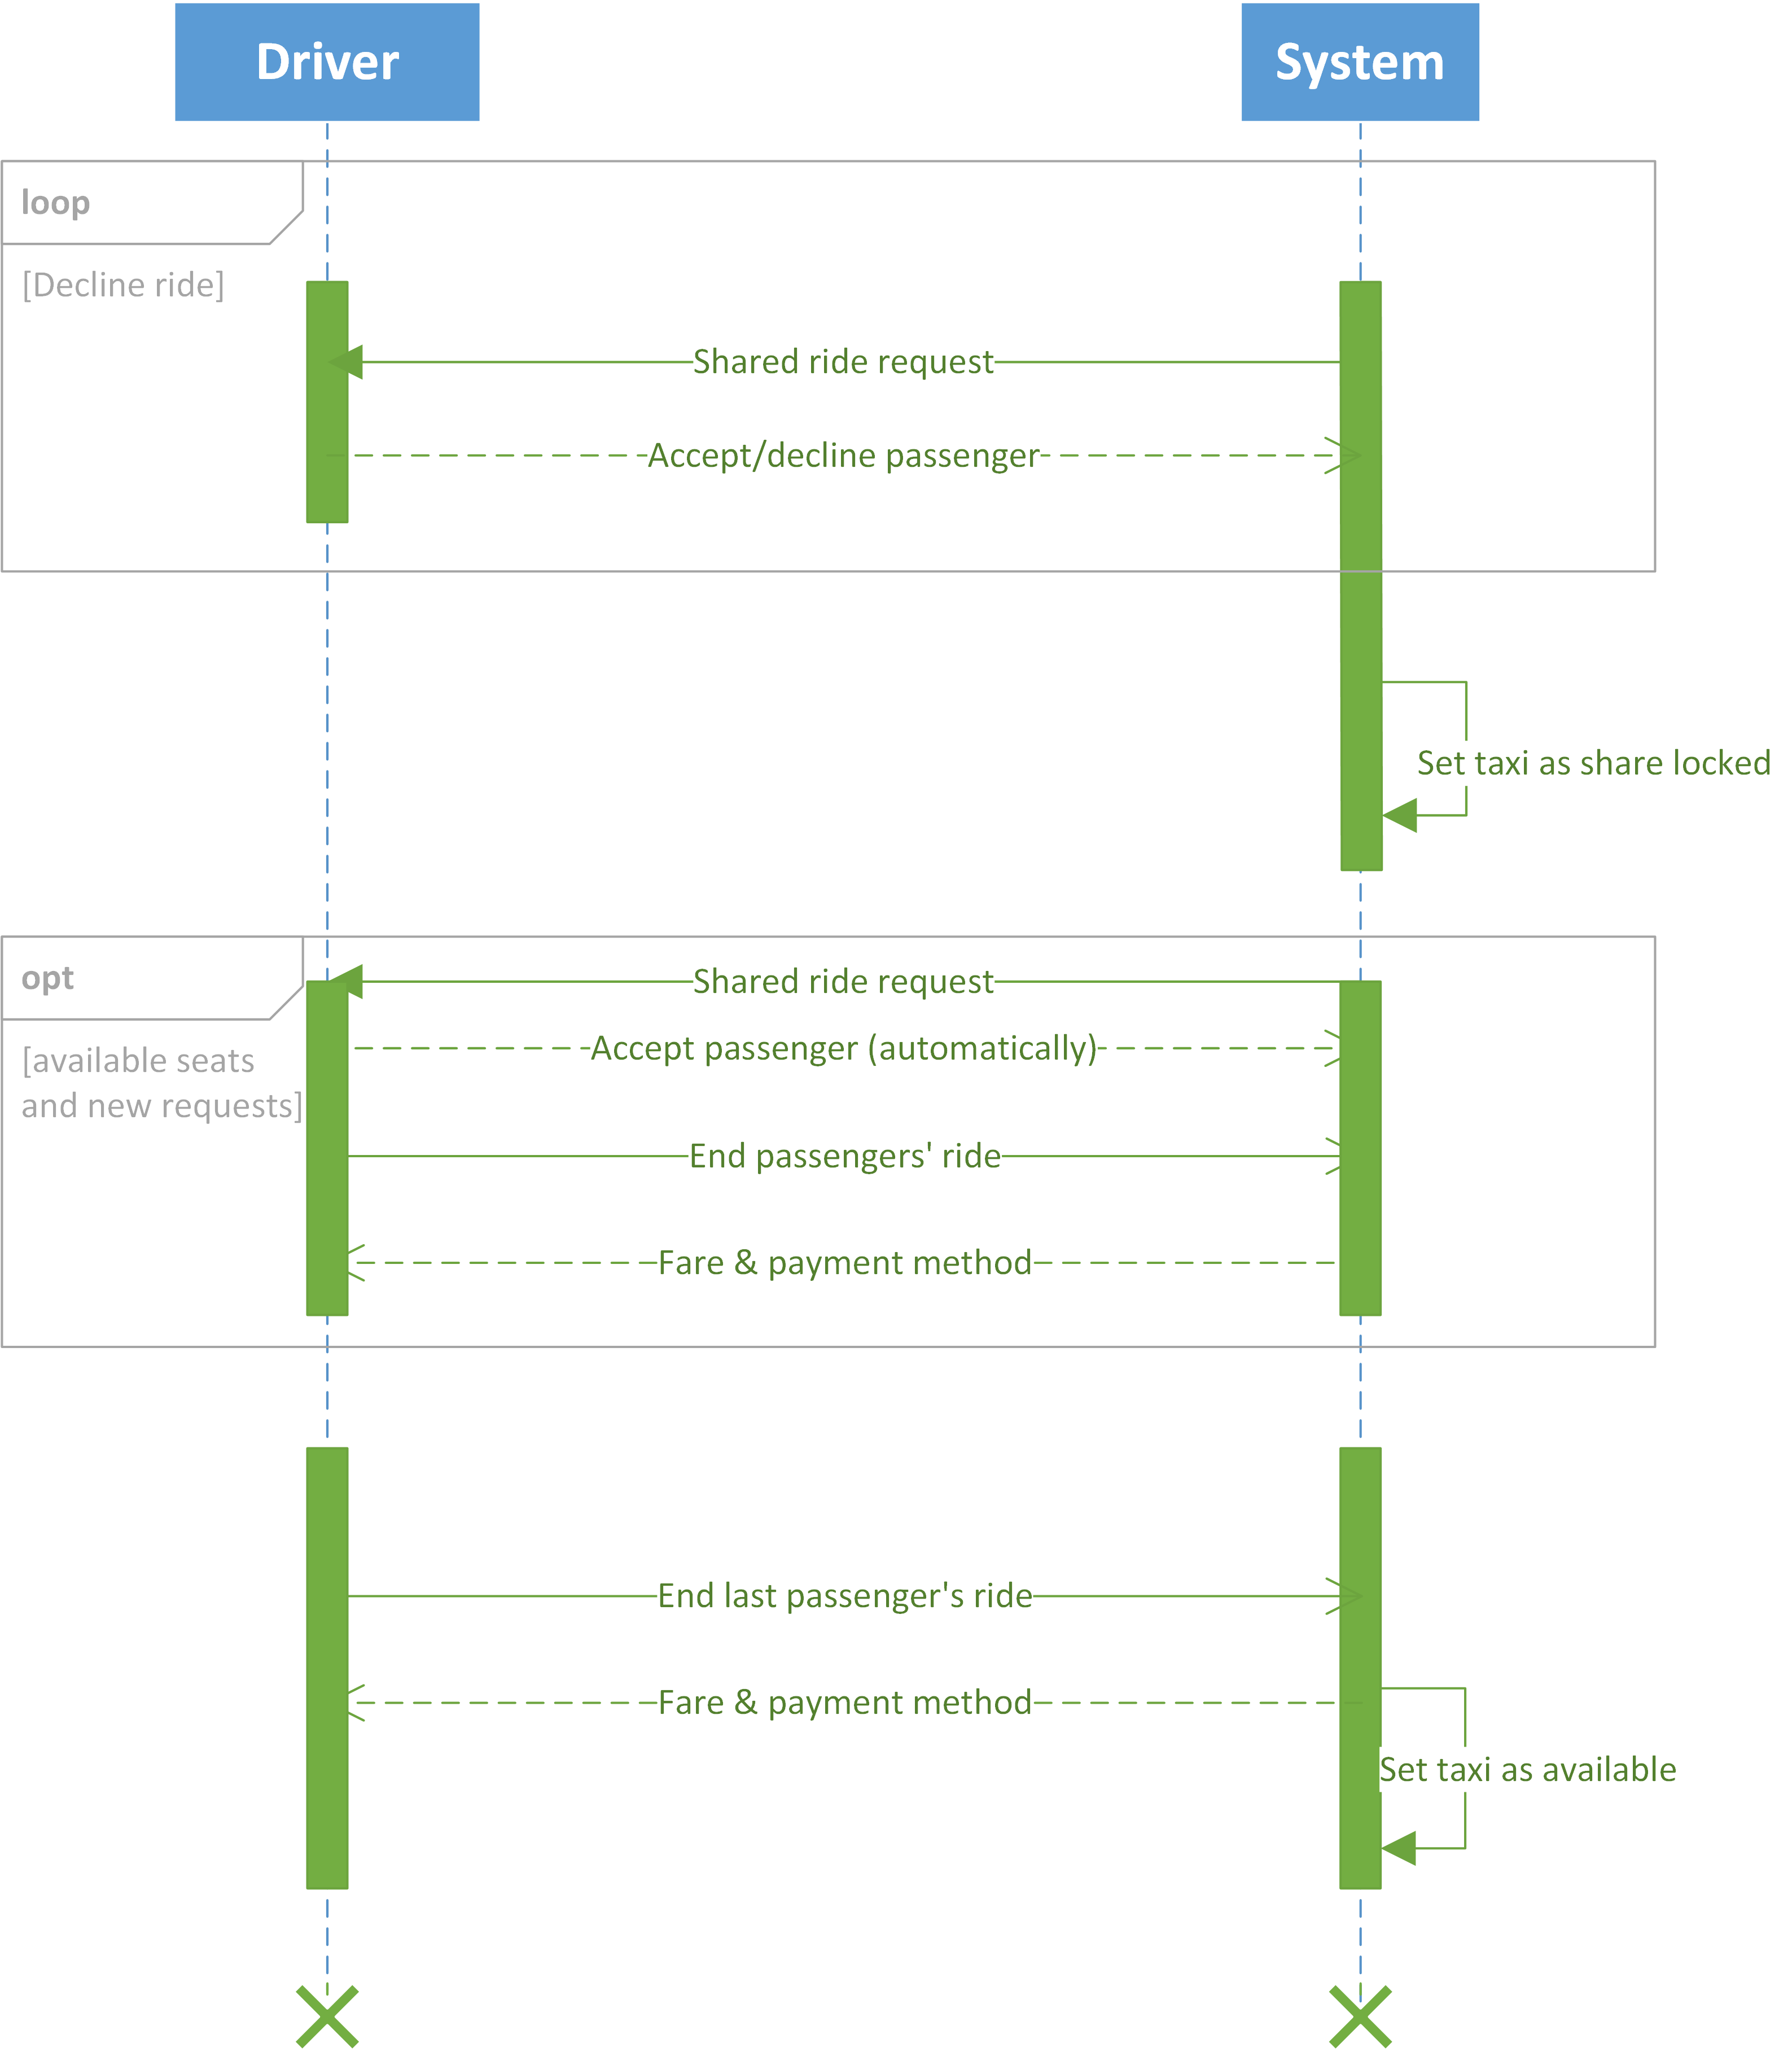
\includegraphics[width=1\columnwidth]{sequenceDiagram/shared-driver}
        \caption{Ride management process - Use case 4.3.8/9}
        \label{fig:seq-shdr}
    \end{figure}

\clearpage

\section{Appendix}

\subsection{Class Diagram}
\begin{figure}[h!]
        \centering
        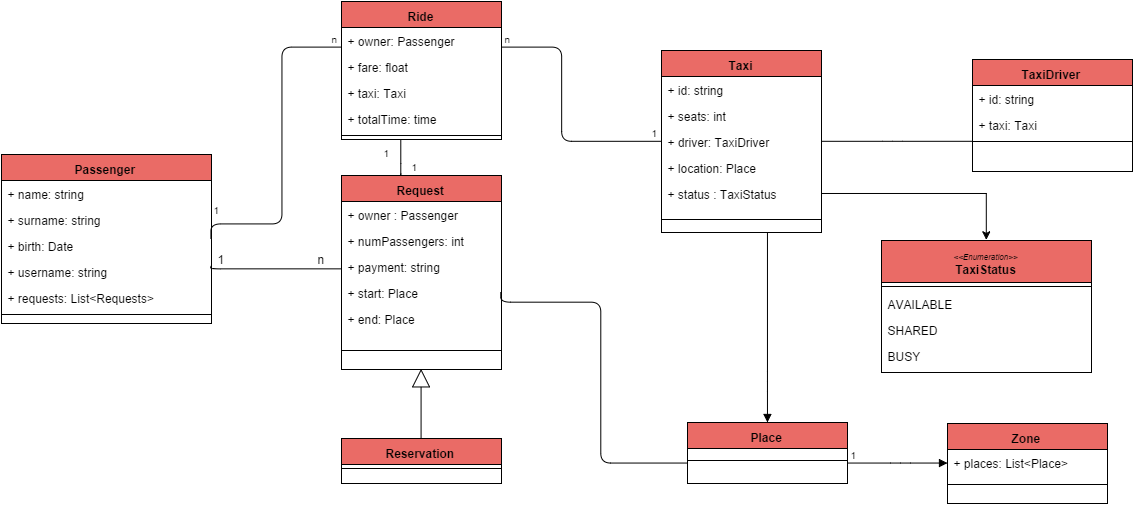
\includegraphics[width=1\columnwidth]{classDiagram/Class-Diagram}
        \caption{Simplified Class Diagram of main entities}
        \label{fig:class-diagram}
    \end{figure}

\newpage

\subsection{Statechart Diagram}

    \begin{figure}[h!]
        \centering
        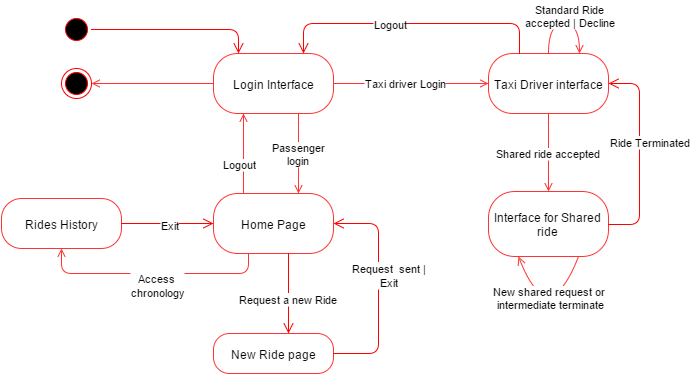
\includegraphics[width=1\columnwidth]{Statechart}
        \label{fig:statechart}
    \end{figure}

\newpage

\subsection{Alloy}
\subsubsection{Purpose}
The Alloy language has been used for its original purpose, which is \textit{model finding}. 
For this sake, in an iterative way we started from a basic class diagram and basic goals 
and requirements we could think at the beginning and we improved and extended them based on 
alloy worlds results.
\subsubsection{Code}
\begin{figure}[h!]
        \centering
        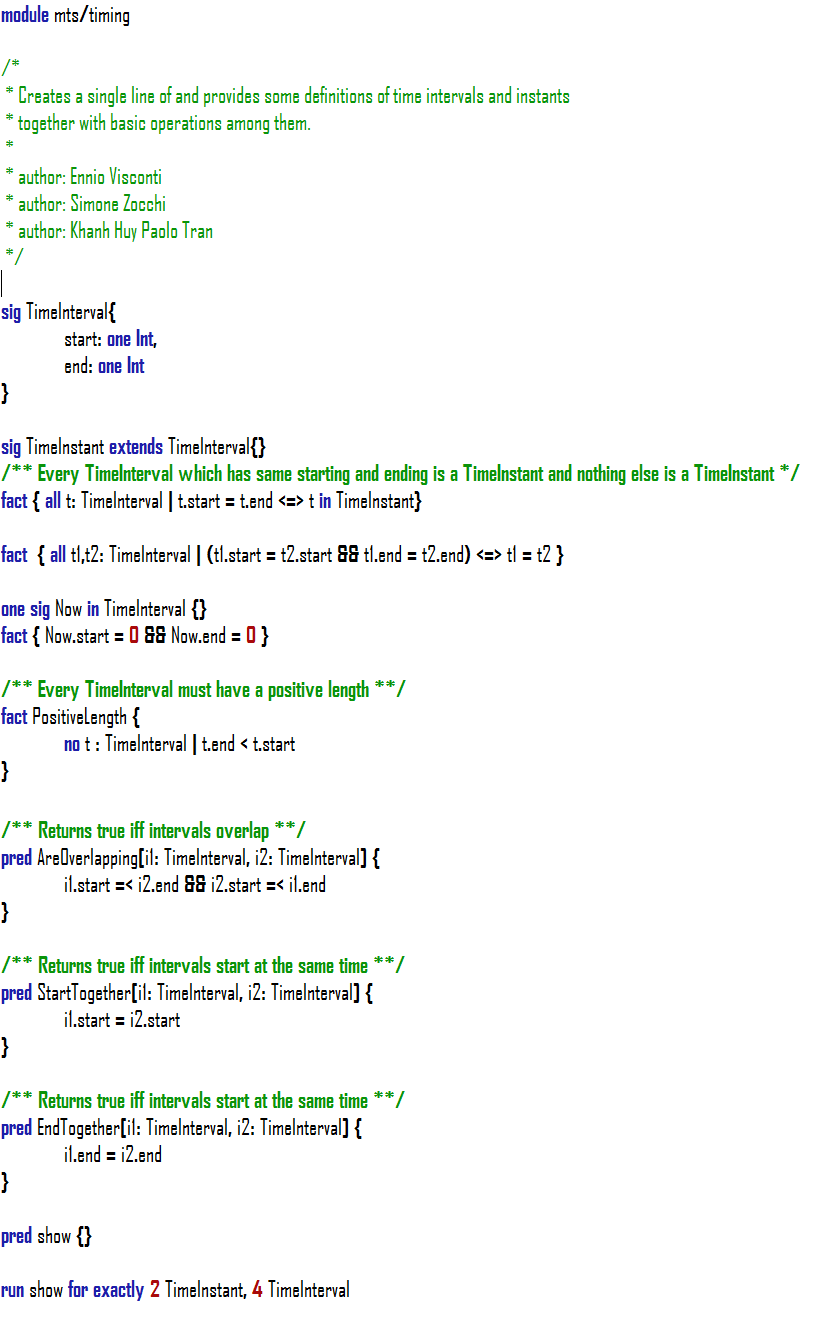
\includegraphics[width=0.85\columnwidth]{alloy/timing}
        \caption{The Alloy library "timing" built to support time requirements}
        \label{fig:alloy-timing}
    \end{figure}
    
\begin{figure}[h!]
        \centering
        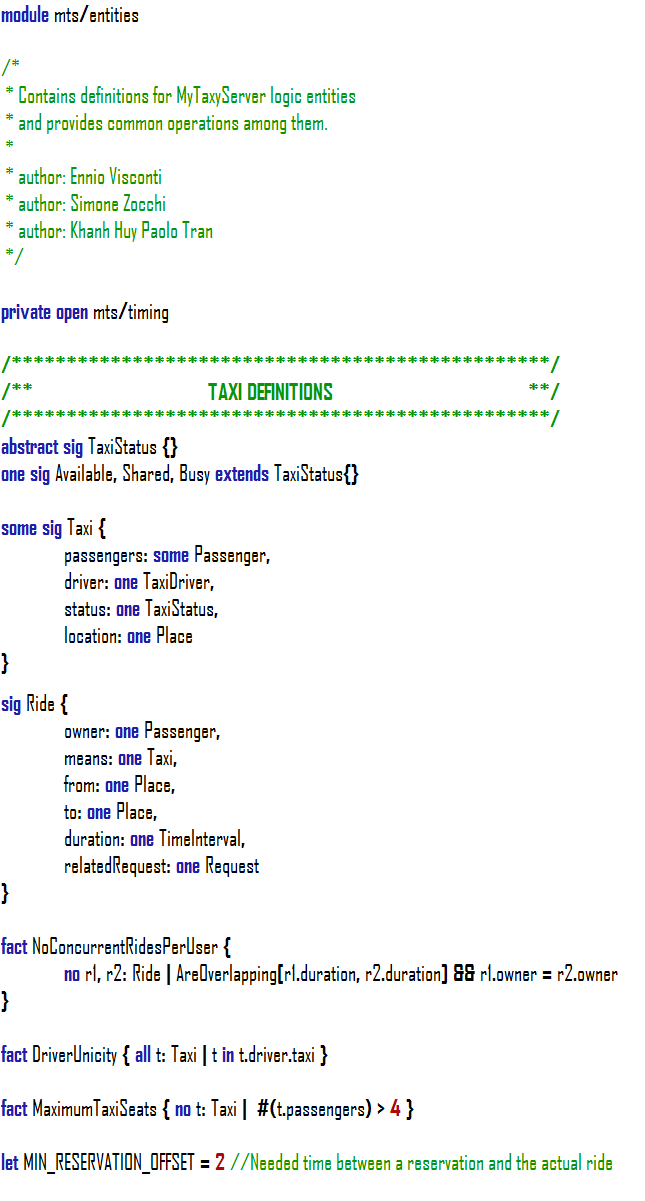
\includegraphics[width=0.8\columnwidth]{alloy/entities1}
        \caption{The Alloy library "entities" built to define basic entities and domain constraints. Part 1}
        \label{fig:alloy-entities-1}
    \end{figure}
    
\begin{figure}[h!]
        \centering
        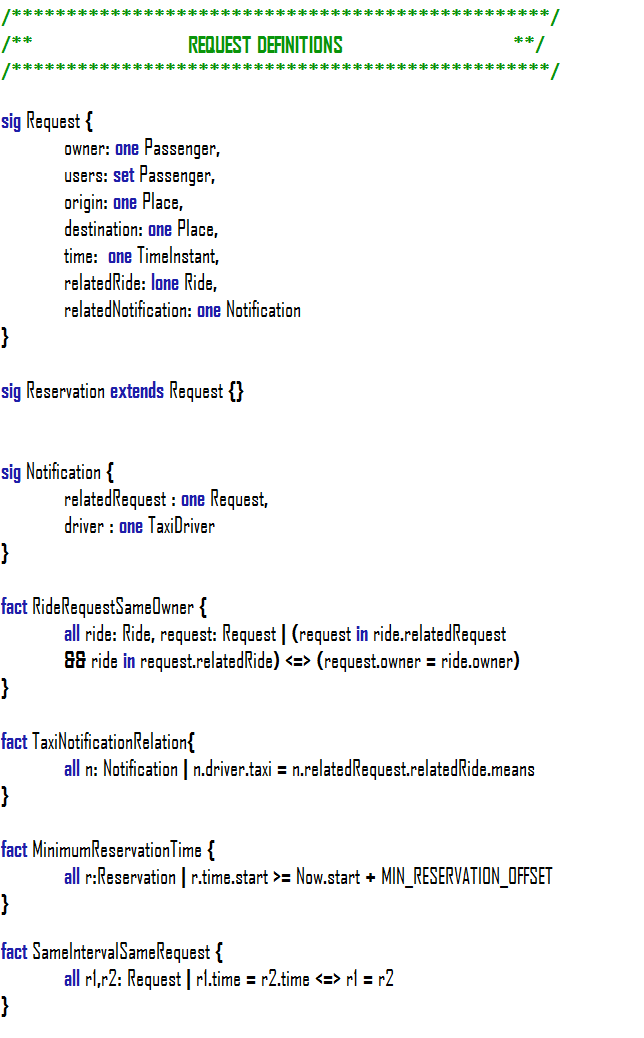
\includegraphics[width=0.9\columnwidth]{alloy/entities2}
        \caption{The Alloy library "entities" built to define basic entities and domain constraints. Part 2}
        \label{fig:alloy-entities-2}
    \end{figure}
    
\begin{figure}[h!]
        \centering
        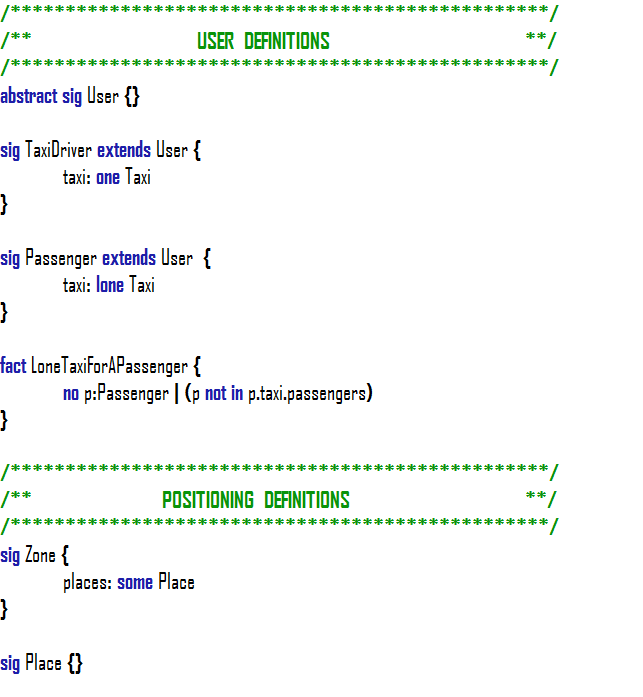
\includegraphics[width=1\columnwidth]{alloy/entities3}
        \caption{The Alloy library "entities" built to define basic entities and domain constraints. Part 3}
        \label{fig:alloy-entities-3}
    \end{figure}
    
\begin{figure}[h!]
        \centering
        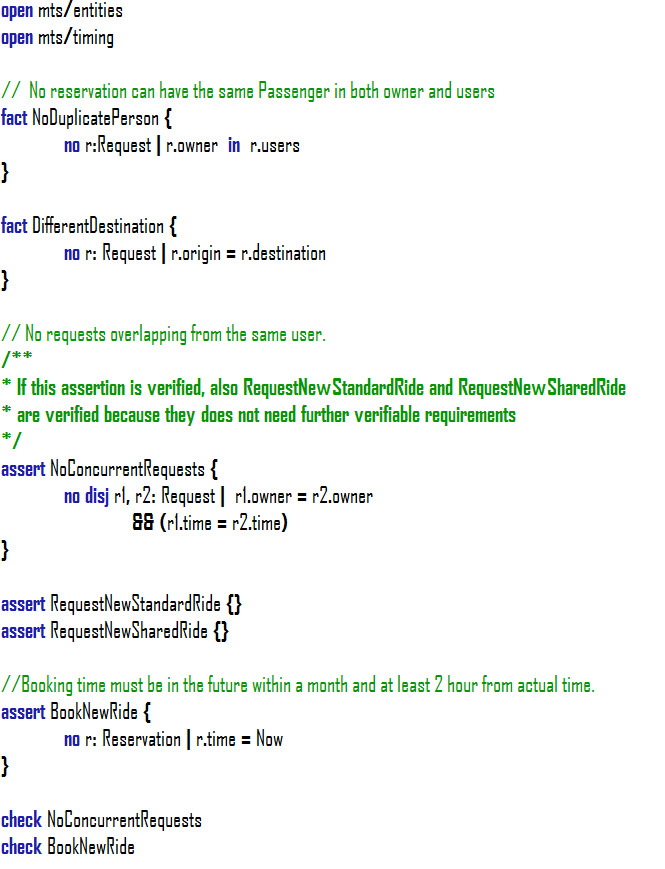
\includegraphics[width=1\columnwidth]{alloy/UC-Passenger}
        \caption{The Alloy requirements assertions and checks based on the Passenger User Class}
        \label{fig:alloy-passenger}
    \end{figure}
    
\begin{figure}[h!]
        \centering
        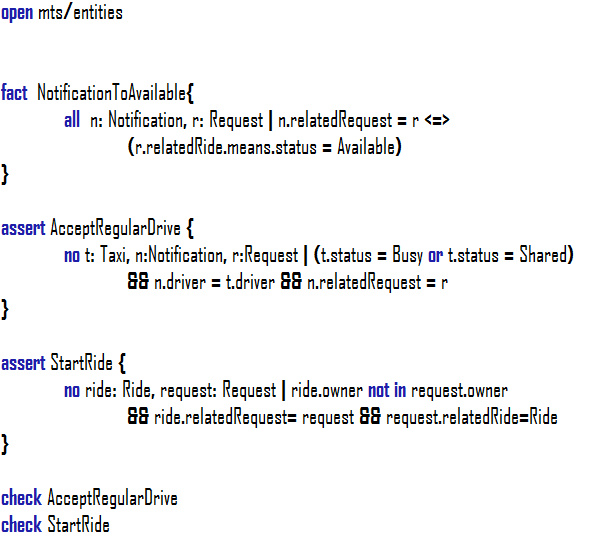
\includegraphics[width=1\columnwidth]{alloy/UC-TaxiDriver}
        \caption{The Alloy requirements assertions and checks based on the Taxi Driver User Class}
        \label{fig:alloy-taxidriver}
    \end{figure}
    
\begin{figure}[h!]
        \centering
        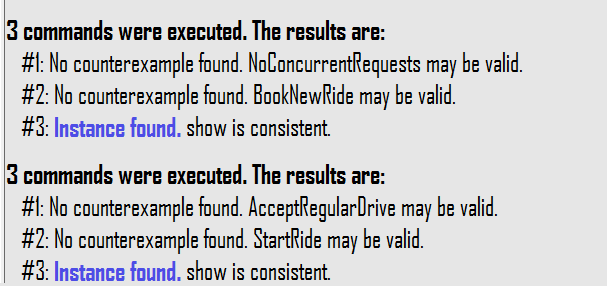
\includegraphics[width=1\columnwidth]{alloy/execution}
        \caption{The Alloy run results}
        \label{fig:alloy-execution}
    \end{figure}
    
\clearpage

\begin{landscape}

\subsubsection{Example Worlds}


\begin{figure}[h!]
        \centering
        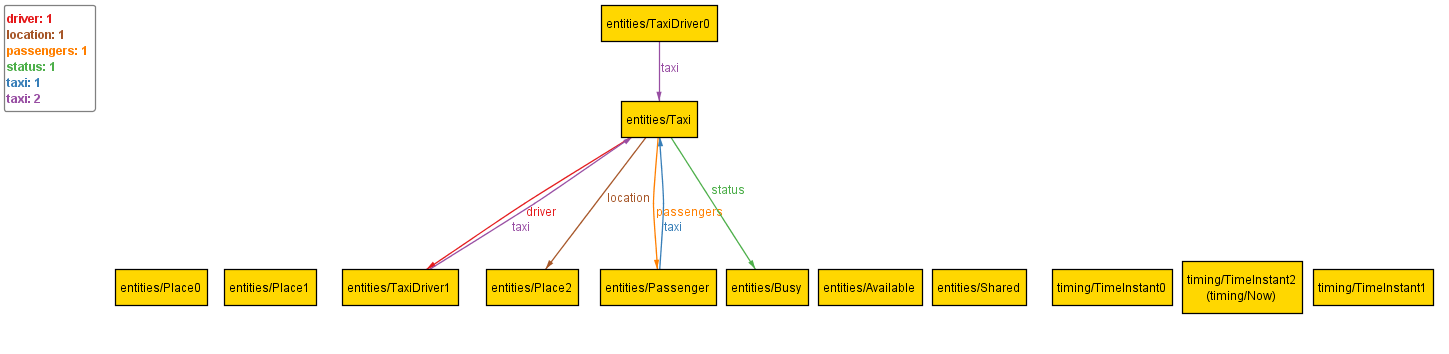
\includegraphics[width=1\columnwidth]{alloy/passenger-world}
        \caption{An Alloy passenger's world}
        \label{fig:alloy-passenger-world}
    \end{figure}
    
\begin{figure}[h!]
        \centering
        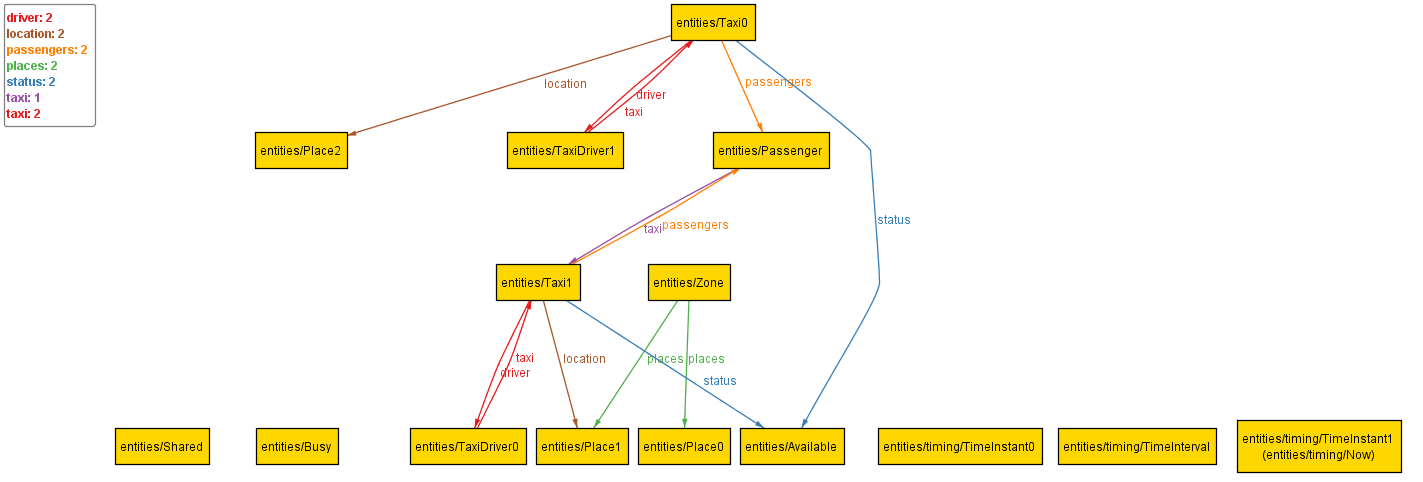
\includegraphics[width=1\columnwidth]{alloy/taxi-driver-world}
        \caption{An Alloy taxi driver's world}
        \label{fig:alloy-taxi-driver-world}
    \end{figure}

\end{landscape}

\end{document}

